\chapter{Desarrollo} \label{development}
En este capítulo se describe la aplicación web eFuel con sus módulos y funcionalidades, luego se narra cómo fue el desarrollo del proyecto. El desarrollo se divide en 3 fases: una fase de inducción donde el pasante se familiarizó con las herramientas y tecnologías necesarias para realizar el proyecto, una fase de desarrollo que consta de 6 Iteraciones de Scrum y una última fase de documentación.

A continuación la descripción de la aplicación seguido de las fases del desarrollo de la misma durante el proyecto de pasantía.

\section{La aplicación web eFuel}
Para este proyecto se desea desarrollar una nueva versión de la aplicación web eFuel basada en tecnologías modernas como ASP.NET y Umbraco. No se usó código de la primera versión, se partió desde cero a programar la nueva versión. Se usaron documentos de la versión original para guiar el desarrollo de la nueva versión de eFuel, especialmente en el diseño de las entidades de la base datos y en las funcionalidades generales (módulos) del sistema.

\subsection{Nueva versión de eFuel}
La nueva versión de eFuel desarrollada para este proyecto es una aplicación web que permite a las estaciones de servicio de combustible la colocación de sus pedidos al mayorista. La aplicación permite consultar información del estado de los pedidos (si fueron despachados y si fueron pagados), asociar facturas a pedidos y asociar pagos a facturas, también permite consultar información sobre otras entidades del dominio de negocio como clientes (estaciones de servicio), transportes disponibles según la zona del cliente, productos disponibles y sus precios. Además, permite importar y exportar información para intercambiar con el \ac{ERP} del mayorista y, de esta manera, servir como sistema de apoyo para este.

\subsubsection{Módulos de funcionalidad}
El sistema se descompone en 4 módulos de funcionalidad: Pedidos, Pagos, Administración y Seguridad. A continuación una breve descripción de las funcionalidades de cada módulo:

\begin{itemize}
    \item \emph{Pedidos}: módulo para la gestión de pedidos. Al crear un pedido se brinda la facilidad de seleccionar rápidamente la combinación de cliente-fecha-turno-transporte-productos. También permite mostrar un listado de los pedidos, filtrar la lista por cliente, transporte, rango de fecha o estado, y luego exportarla como un archivo de Excel. 
    \item \emph{Pagos}: módulo para la gestión de pagos y facturas. Con este módulo se pueden importar facturas desde un archivo de Excel generado por el \ac{ERP} del mayorista, éstas se asocian inmediatamente con un pedido. También se pueden gestionar los pagos, asociar pagos a facturas y exportarlos a un archivo de Excel.
    \item \emph{Administración}: módulo para la gestión de clientes, transportes, productos, zonas y turnos. Esto incluye creación, edición, consulta, listado, importación y eliminación de estas entidades del sistema.
    \item \emph{Seguridad}: este módulo controla el acceso a la aplicación para garantizar que únicamente las personas autorizadas puedan consultar los datos y realizar las operaciones que les corresponden. Se pueden crear y editar miebros, así como modificar los permisos de cada uno.
\end{itemize}

\subsubsection{Sobre los modelos de datos}
Las entidades del sistema las podemos dividir en 2 categorías: transaccionales y no transaccionales. Las entidades transaccionales son objetos que se van a generar con mucha frequencia durante el funcionamiento del sistema: pedidos, facturas y cobros; las no transaccionales no se generan con tanta frequencia: clientes, transportes, zonas, turnos y productos.

Al crear un nodo de contenido desde el back office de Umbraco se guarda cierta información adicional a las propiedades definidas por el programador: fechas de publicación, versiones, autor, entre otras. Esto no es conveniente para modelar las entidades transaccionales ya que se genera un volumen importante de éstas y mucha de esa información adicional no es necesaria. Por esta razón, se decidió modelar las entidades transaccionales como tablas en la base de datos independientes de las tablas de Umbraco las entidades no transaccionales se modelaron como Doctypes de Umbraco, que son definiciones de la estructura de un tipo de contenido (para más detalles ver la Sección \ref{conceptosUmbraco}).

En la Figura \ref{fig:esquema_general_nuevo} se muestra el esquema general del sistema.

\vspace{0.3cm}

\begin{figure}[ht]
    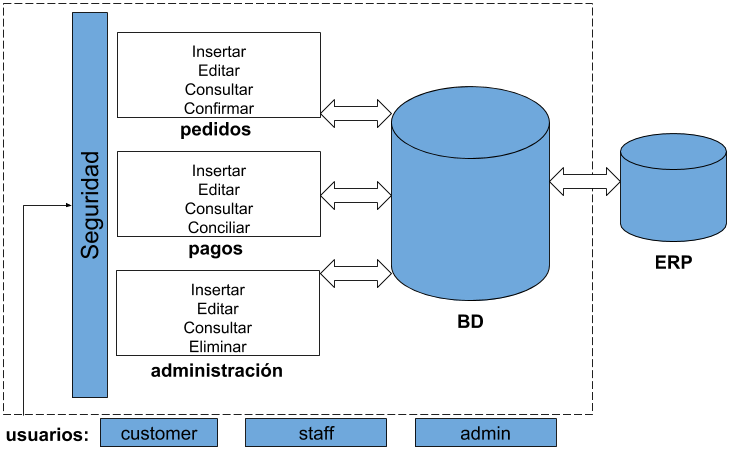
\includegraphics[width=\textwidth]{esquema_general_nuevo.png}
    \caption{Esquema general de los módulos de funcionalidad}
    \label{fig:esquema_general_nuevo}
    \centering
\end{figure}

Uno de los objetivos de la aplicación es servir como sistema de apoyo a los ERP de los mayoristas. Los sistemas ERP llevan el control de todas las entidades del negocio, entre estas están las estaciones de servicio, los transportes para los pedidos, los pedidos, las facturas, etc. La aplicación eFuel interactúa con el \ac{ERP} y le sirve de apoyo a éste manteniendo un registro separado de las entidades pertinentes a la inserción y el pago de pedidos de combustible. Esta interacción se da a través de importaciones y exportaciones de datos entre estos sistemas para que estén sincronizados.

\section{Fases del desarrollo}
\subsection{Fase de Inducción}
Esta fase tuvo una duración de 1 semana, el pasante realizó varios tutoriales y utilizó varios recursos (guías de Umbraco, videos de ASP.NET, entre otros) proporcionados por la empresa para inducir los conocimientos técnicos necesarios para llevar a cabo el proyecto. Las herramientas investigadas fueron: Umbraco, ASP.NET, SQL Server y Visual Studio.

\subsection{Fase de Desarrollo}
Esta fase duró 16 semanas continuas y se llevaron a cabo 6 Iteraciones donde se desarrolló la aplicación. A continuación una descripción del trabajo realizado en cada iteración.

\subsubsection{Análisis de requerimientos (1era Iteración)}
Se definió la arquitectura y la estructura de la base de datos. Además, se creó el repositorio de Git, el proyecto de Visual Studio y el sitio de Umbraco, y por otro lado, se eligió una plantilla de HTML para el \emph{look and feel} de la aplicación.

\vspace{0.3cm}
\textbf{Actividades realizadas:}
\begin{itemize}
    \item El pasante se familiarizó con la versión original de eFuel.
    \item El pasante se familiarizó con las reglas de negocio.
    \item El pasante junto con el dueño del producto definieron los actores del sistema, estos son: \emph{admin} (adminsitradores del sistema), \emph{staff} (empleados del mayorista) y \emph{customer} (empleados de las estaciones de servicio).
    \item Se listaron las funcionalidades básicas del front end a desarrollar. Esta lista de funcionalidades fue refinada y expandida a medida que se avanzo con el desarrollo. Listado de funcionalidades básicas elaborado:
        \begin{itemize}
            \item Listado de pedidos.
            \item Creación de pedidos.
            \item Listado de clientes, zonas y transportes.
            \item Listado de facturas.
        \end{itemize}
    \item Creación de la solución de Visual Studio con los módulos \texttt{EF\_Core}, \texttt{EF\_Core} y \texttt{EF\_\-Miscelaneous}.
    \item Creación del repositorio de Git y familiarización con las reglas del mismo.
    \item Se definieron las entidades de la base de datos del proyecto para poder implementar funcionalidades básicas del sistema. Esto incluyó decidir qué entidades se modelarán como tablas en la base datos directamente y qué entidades se modelarán como Doctypes de Umbraco. Finalmente se definieron las columnas que tienen las tablas de la base de datos.
    \item Se creó el sitio de Umbraco.
    \item Se evaluaron 2 plantillas de HTML para el estilo del sitio, ambas eran plantillas de tableros o \emph{dashboards}, se decidió utilizar una plantilla gratuita llamada Adminator, en la Figura \ref{fig:orderslist} se muestra una captura de la plantilla elegida.
\end{itemize}

\begin{figure}[H]
    \centering
    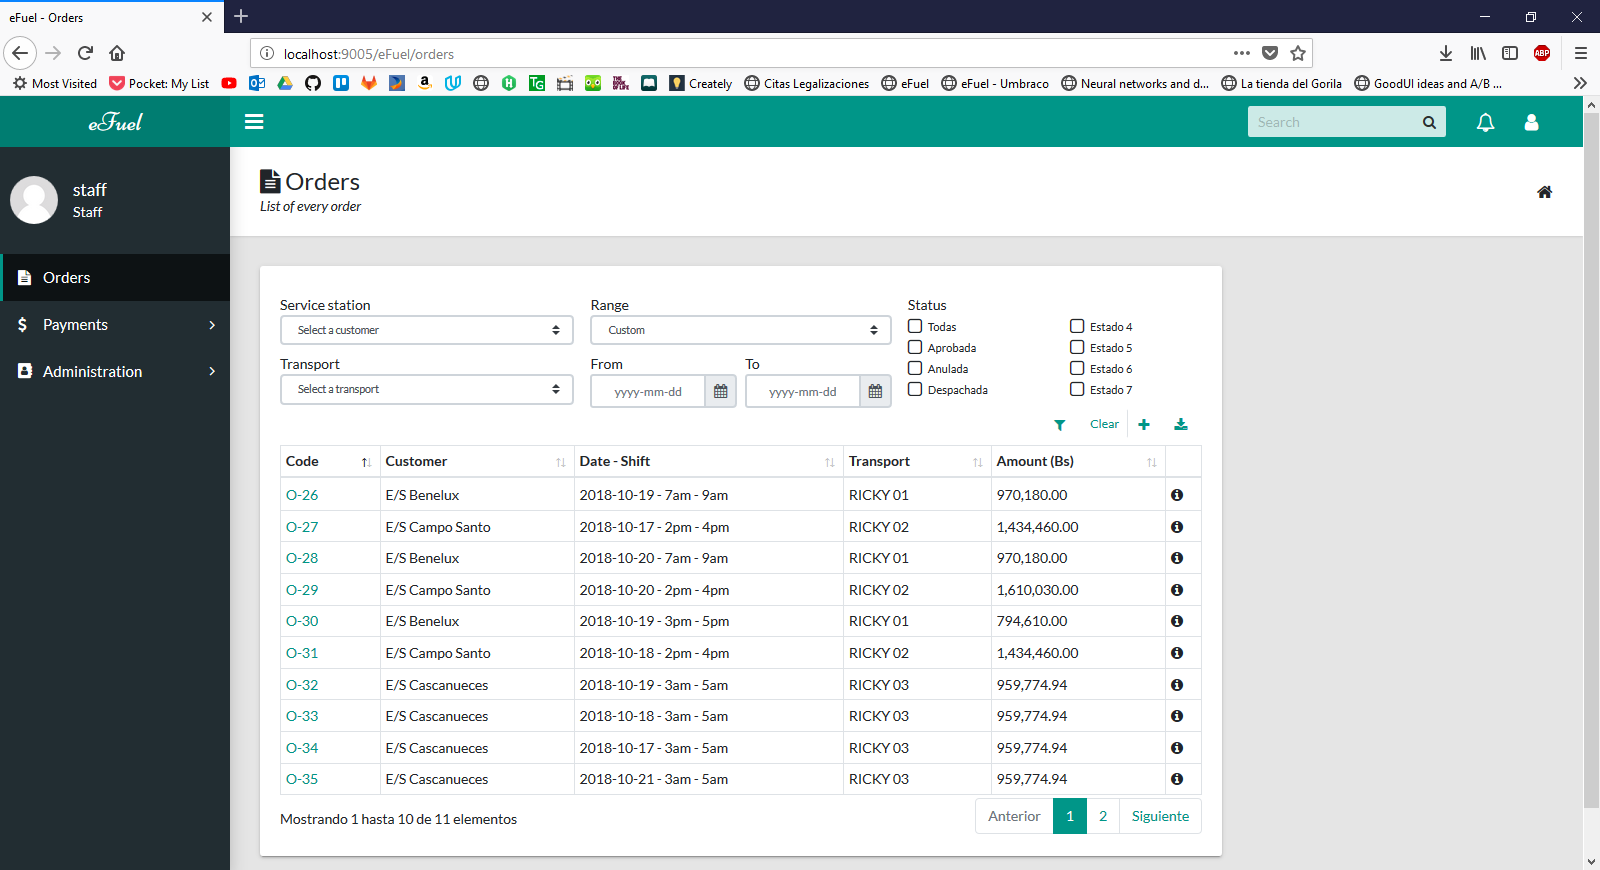
\includegraphics[width=0.7\textwidth]{./vistas/frontend/orders_list.png}
    \caption{Lista de pedidos (captura)}
    \label{fig:orderslist}
\end{figure}

\textbf{Duración:} 2 semanas.

\subsubsection{Módulo de Administración (2da Iteración)}
Se implementó la funcionalidad de manejo de las entidades principales de la aplicación: clientes, productos, transportes, zonas, turnos, pedidos, facturas y cobros. Para esto se implementó una interfaz en el back end de Umbraco usando Fluidity y se definieron los Doctypes y Data Types de las entidades a ser almacenadas como contenido de Umbraco.

También se empezó el desarrollo del front end de la aplicación. Al finalizar esta Iteración se tuvo una forma de manejar las entidades del sistema, ya sea a través del árbol de contenido de Umbraco o a través de la interfaz de Fluidity.

\vspace{0.3cm}
\textbf{Actividades realizadas:}
\begin{itemize}
    \item Se diseñaron los Doctypes y Data Types para las entidades no transaccionales (clientes, transportes, zonas, turnos y productos).
    \item Se desarrolló la interfaz de Fluidity para insertar registros en la base de datos de las entidades transaccionales. Esta actividad se realizó para tener una manera de gestionar las entidades transaccionales mientras no se tenga implementada esta funcionalidad en el front end.
    \item Se empezó el desarrollo de la barra de navegación, títulos de las páginas, menú de navegación para el front end. Éstos son elementos que tienen en común la mayoría de las vistas del front end.
    \item Se implementó la funcionalidad de listado de clientes en el front end. Primero se desarrolló el controlador para mostrar la vista y luego se diseñó la vista (el archivo de HTML). Se implementaron 2 controladores: uno de tipo \texttt{UmbracoApiController} para devolver los elementos de la lista y otro de tipo \texttt{SurfaceController} para devolver la vista como tal. También se desarrolló un script de JavaScript para manejar la organización de las tablas usando Datatables.
    \item Se implementó la funcionalidad de detalles de un cliente en el front end, se diseñaron el controlador y la vista correspondientes.
\end{itemize}

\textbf{Duración:} 3 semanas.

\subsubsection{Módulo de Administración (cont.) y Pedidos (3ra Iteración)}
Esta Iteración estuvo dedicada a terminar algunas funcionalidades del módulo de Administración en el front end y al desarrollo de la funcionalidad referente a los pedidos de combustible. Se desarrolló el listado de pedido con filtros, el formulario de creación de pedidos y la exportación de la lista de pedidos.

\pagebreak
\textbf{Actividades realizadas:}
\begin{itemize}
    \item Se implementaron las funcionalidades de listado de transportes y zonas en el front end. Para esto se diseñaron los controladores, las vistas y los scripts de JavaScript correspondientes.
    \item Se implementó la funcionalidad de listado de pedidos en el front end. Se diseñaron los controladores para devolver los datos de los pedidos y para devolver la vista, además se diseñó la vista de listado de pedidos y el script de JavaScript para manejar la tabla.
    \item Se implementó la funcionalidad de filtrado para la lista de pedidos en el front end. Para esto se modificó el archivo de JavaScript encargado de manejar la tabla para que también manejara los filtros aplicados a ésta y se agregaron varios métodos al controlador que devuelve la lista de pedidos. Cada método se encarga de seleccionar los pedidos de una lista de pedidos que tengan el mismo valor que el filtro deseado por el cliente en alguna propiedad. Hay un método por cada propiedad de los pedidos.
    \item Se implementó la funcionalidad de consultar los detalles de un pedido en el front end. Para esto se diseñaron el controlador y la vista correspondientes.
\end{itemize}

\textbf{Duración:} 2 semanas.

\subsubsection{Refactorización (4ta Iteración)} \label{refactorizacion}
Al realizar una revisión de la estructura del código se determinó que éste debía ser refactorizado para seguir el patrón MVC enforzado por ASP.NET MVC, de esta manera el código se haría más fácil de mantener y extender al aprovechar las virtudes del patrón MVC.

Hasta ese punto del desarrollo los Controladores no reflejaban adecuadamente la estructura MVC y por lo tanto no se aprovechaba al máximo las vistudes de este patrón. Se habían implementado Controladores para cada "tipo" de funcionalidad, por ejemplo, en el caso de los pedidos había 3 Controladores: \texttt{OrdersController} que devolvía la lista de pedidos, \texttt{OrderDetailController} que devolvía la vista de detalles y \texttt{NewOrderFormContro\-ller} que devolvía el formulario para crear un nuevo pedido y procesaba la información de éste. Al utilizar esta estructura se generó una elevada cantidad de archivos (uno por Controlador), éstos se agruparon en carpetas por Modelos, de esta manera los 3 Controladores que se encargaban de la lista, los detalles y crear un pedido se juntaban en una carpeta llamada \texttt{Orders}. El resultado fue código díficil de mantener (por la cantidad de archivos) y que no seguía las buenas prácticas sugeridas por el diseño de ASP.NET MVC.

Para resolver estos inconvenientes y mejorar la calidad del código se agrupó la funcionalidad según los Modelos: existe un Controlador para cada Modelo y los \emph{métodos} del Controlador implementan la funcionalidad. Siguiendo con el ejemplo de los pedidos, en vez de tener un Controlador para cada acción, se tiene un Controlador \texttt{OrderController} asociado al Modelo de Pedido que contiene los métodos \texttt{List}, \texttt{Detail} y \texttt{Create}, cada uno de estos métodos implementa una acción específica, de esta manera toda la funcionalidad referente a los pedidos se encuentra en un archivo. Con este esquema también se ve claramente qué acciones se pueden llevar a cabo sobre el Modelo.

Por otro lado, las Vistas de la aplicación también se organizaron siguiendo el patrón MVC. Hay una carpeta para cada Modelo y dentro de ésta hay una vista para cada acción o método que se puede realizar (y que requiera de una vista) sobre este Modelo. Con esta organización se puede ver claramente una correspondencia entre un Modelo, un Controlador y sus Vistas.

A continuación se muestran algunas figuras que ilustran los cambios realizados, siguiendo el ejemplo descrito en los párrafos anteriores:

\begin{figure}[H]
    \centering
    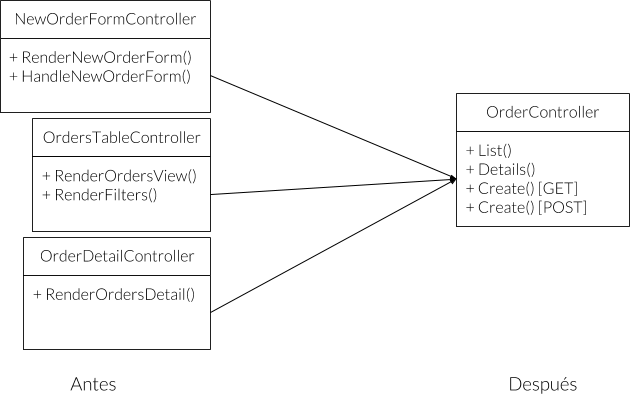
\includegraphics[width=0.7\textwidth]{controller_changes.png}
    \caption{Cambios a los controladores}
    \label{fig:controller_changes}
\end{figure}

\begin{figure}[H]
    \centering
    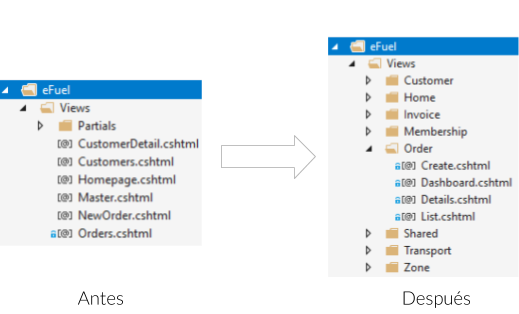
\includegraphics[width=0.7\textwidth]{views_changes.png}
    \caption{Cambios a las vistas}
    \label{fig:views_changes}
\end{figure}

Durante esta iteración también se llevó a cabo una reunión con los miembros del equipo (el dueño del producto/tutor industrial y otros integrantes del equipo de programación de la empresa) para revisar el estado de la aplicación y para evaluar el código escrito hasta el momento. Como resultado de la evaluación se realizaron varios comentarios y correcciones sobre el código para seguir las buenas prácticas y convenciones del equipo de desarrollo de la empresa.

\vspace{0.3cm}
\textbf{Actividades realizadas:}
\begin{itemize}
    \item Se cambió la estructura del código para que siguiera el patrón MVC de una mejor manera.
    \item Mejoras en la calidad del código en general. Se hizo más robusto el código al chequear cada conexión a la base de datos para capturar errores, se mejoró la eficiencia de algunas consultas a la base de datos, se cambiaron los nombres de algunas variables y métodos, se ajustaron algunos detalles con el espacado del código. Todo esto con el objetivo de seguir las buenas prácticas de la empresa y hacer el código más legible y mantenible.
\end{itemize}

\textbf{Duración:} 3 semanas.

\subsubsection{Continuación con el Módulo de Pedidos (5ta Iteración)}
En esta Iteración se continuó el desarrollo de la funcionalidad referente a los pedidos del sistema.

\vspace{0.3cm}
\textbf{Actividades realizadas:}
\begin{itemize}
    \item Implementación de la funcionalidad de crear pedido en el front end. Para esto fue necesario crear 2 métodos en el controlador de pedidos, un para mostrar el formulario y otro para chequear que los datos introducidos son válidos, también se implementó un método que, dado un cliente, devuelve la lista de fechas disponibles con los transportes y turnos disponibles. También se diseñó la vista correspondiente y se desarrolló un script de JavaScript para ir hablitando los campos del formulario a medida que se van seleccionando las opciones. Para crear un pedido se debe selccionar un cliente, al seleccionarlo el servidor envía al cliente la lista de fechas disponibles con sus transportes y turnos correspondientes, se habilita el campo de fecha, se seleccicona una fecha, se habilita el campo de transporte y se selecciona uno de los transportes disponibles, se habilita el campo de turno, se selcciona uno de los disponibles y, fianlmente se selccionan los productos del pedido. En la Figura \ref{fig:ordercreate} se muestra el formulario.
    \item Implementación de la funcionalidad exportación de la lista de pedidos desde el front end. Para esto se diseñó un método que busca la lista de pedidos (puede o no tener filtros aplicados) y genera un archivo de Excel con la información de éstos.
\end{itemize}

\begin{figure}[H]
    \centering
    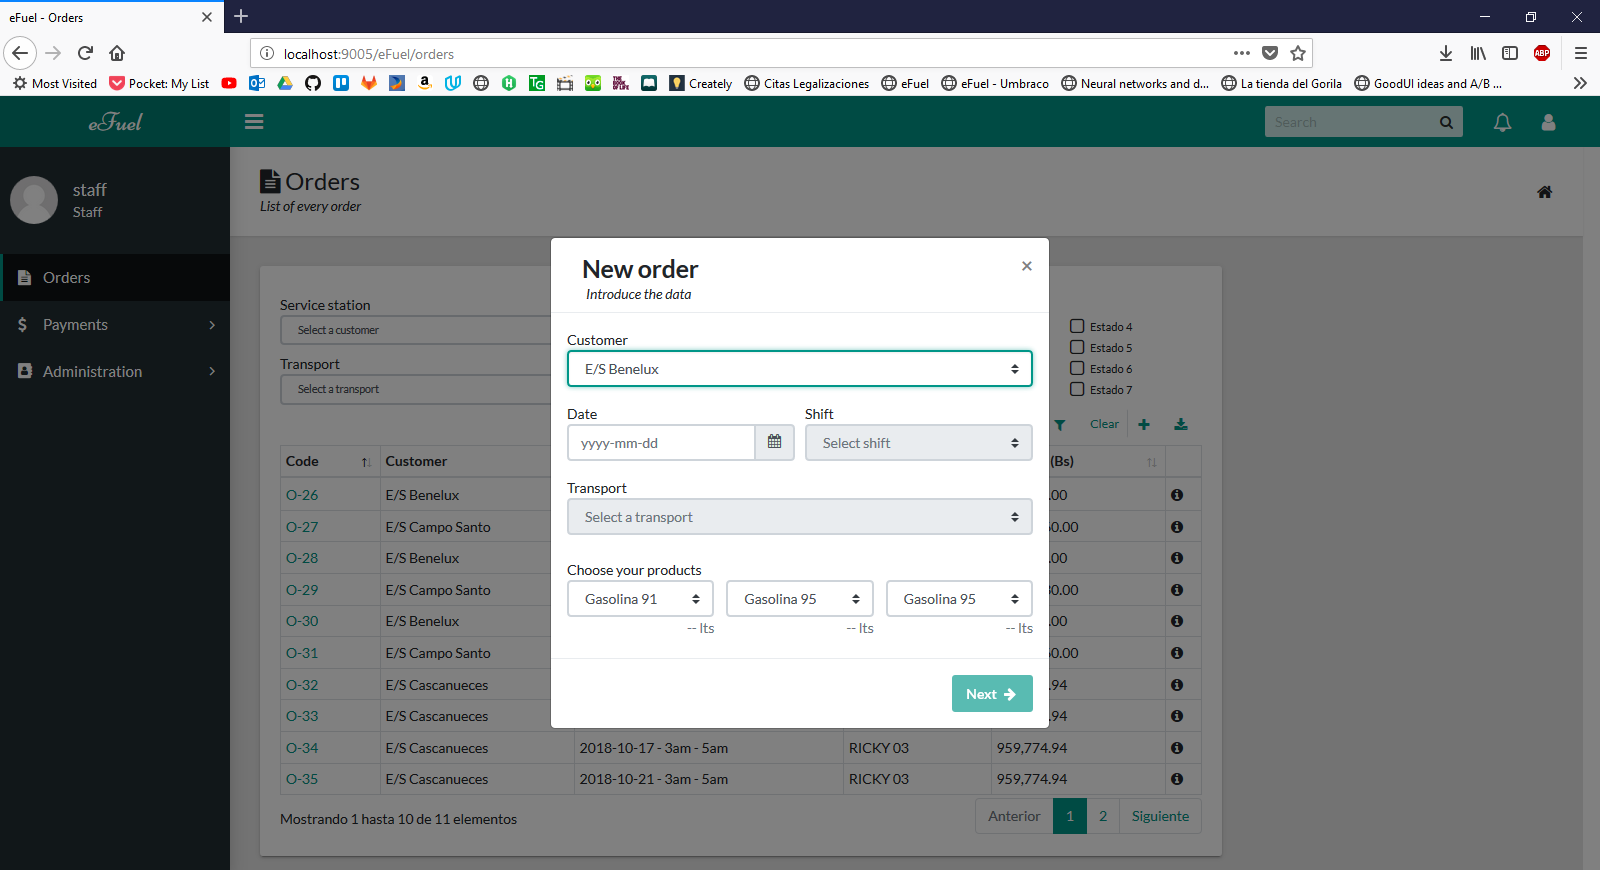
\includegraphics[width=0.7\textwidth]{./vistas/frontend/orders_create.png}
    \caption{Formulario para crear un pedido (captura)}
    \label{fig:ordercreate}
\end{figure}

\textbf{Duración:} 3 semanas.

\subsubsection{Módulo de Manejo de Usuarios e Importación (6ta Iteración)}
Ésta fue la última Iteración de desarrollo, en ella se desarrolló el módulo de manejo de usuarios y se implementó la funcionalidad de importación de algunas entidades. También se mejoraron todos los aspectos que fueron posibles del código y se empezó a desarrollar el módulo de pagos, tan solo se terminó una vista (lista de facturas).

\vspace{0.3cm}
\textbf{Actividades realizadas:}
\begin{itemize}
    \item Se definieron los tipos de usuario y los permisos por actor (customer y staff) para el front end. Para esto se creó un tipo de miembro llamado \emph{eFuel Member} desde la sección Members del back office de Umraco y luego se crearon 2 grupos de miembros: \emph{eFuel Customer} y \emph{eFuel Staff}.
    \item Implementación de funcionalidad de autenticación, inicio y cierre de sesión para el front end de la aplicación. Para esto se tuvo que agregar lógica de autenticaión en cada método de cada controlador para chequear si hay un usuario con una sesión abierta y, en ese caso, si posee los permisos necesarios.
    \item Implementación de la funcionalidad de importación de Zonas y Transportes desde archivos de Excel en el front end. Para esto se implementaron métodos en los controladores de Transportes y Zonas que se encargan de leer un archivo de Excel y de crear registros en la base de datos basados en la información de los archivos.
    \item Se implementó la funcionalidad de listado de facturas en el front end. Para esto se diseñaron el controlador y la vista correspondientes.
\end{itemize}

\textbf{Duración:} 3 semanas.

\subsection{Fase de Documentación} \label{documentation}
Esta fase duró 1 semana, en ella se elaboró un Documento de Arquitectura de Software donde se detallan los componentes y casos de uso desarrollados de la aplicación y, además, se elaboró una guía de instalación de eFuel.

A continuación se describe la arquitectura del software como aparece en el Documento de Arquitectura del Software desarrollado durante esta fase. El documento está basado en el modelo 4+1 de arquitectura de Phillipe Kruchten \cite{41Kruchten}, contempla la Vista de Casos de Uso, la Vista Lógica, la Vista de Implantación, la Vista de Implementación y la Vista de Datos, adicionalmente se elaboró documentación de los componentes de Umbraco del sistema y se incorporó a este documento. Para una descripción detallada de todas las vistas elaboradas referirse al Anexo \ref{das}.

\subsubsection{Arquitectura de Software}
En esta sección se presentan los elementos importantes cada una de las vistas elaboradas para el Documento de Arquitectura del Software. Referirse al Anexo \ref{das} para ver todos los detalles elaborados.

\paragraph{Vista de Casos de Uso} En esta vista se describirá el sistema desde el punto de vista de los casos de uso. El sistema tiene 3 actores:

\begin{itemize}
    \item \emph{Admin}: administrador de eFuel. Es un usuario de Umbraco, esto es, cuenta con las credenciales para ingresar al back end de Umbraco y, además, tiene los permisos necesarios para administrar las entidades y los miembros de eFuel.
    \item \emph{Customer}: representa a una o varias estaciones de servicio. Solo tiene acceso a la información referente a las estaciones de servicio asignadas por el administrador del sistema. Es el tipo de miembro que más uso le dará al sistema.
    \item \emph{Staff}: representa a un distribuidor de combustible. Tiene acceso a la información de todas las estaciones de servicio del sistema.
\end{itemize}

A continuación, se presenta el resumen de los casos de uso del sistema.

\newcounter{magicrownumbers}
\newcommand\rownumber{\stepcounter{magicrownumbers}\arabic{magicrownumbers}}

\vspace{0.4cm}
\begin{longtable}{ | l | l | c | }
    \hline
    \rowcolor{gray!30}
    \multicolumn{1}{|c|}{ID del Caso de Uso} &
    \multicolumn{1}{|c|}{Caso de Uso} &
    \multicolumn{1}{|c|}{Actor} \\
    \hhline{===}
    \endhead

    CU-\rownumber & Iniciar sesión (Umbraco) & Admin \\ \hline
    CU-\rownumber & Consultar lista de miembros & Admin \\ \hline
    CU-\rownumber & Gestionar miembro (CRUD) & Admin \\ \hline
    CU-\rownumber & Asignar cliente/s a miembro & Admin \\ \hline
    CU-\rownumber & Remover cliente/s de miembro & Admin \\ \hline
    CU-\rownumber & Cambiar permisos de miembro & Admin \\ \hline

    CU-\rownumber & Gestionar contenido & Admin \\ \hline
    CU-\rownumber & Consultar lista de clientes & Admin \\ \hline
    CU-\rownumber & Gestionar cliente (CRUD) & Admin \\ \hline
    CU-\rownumber & Consultar lista de productos & Admin \\ \hline
    CU-\rownumber & Gestionar producto (CRUD) & Admin \\ \hline
    CU-\rownumber & Consultar lista de transportes & Admin \\ \hline
    CU-\rownumber & Gestionar transportes (CRUD) & Admin \\ \hline
    CU-\rownumber & Consultar lista de zonas & Admin \\ \hline
    CU-\rownumber & Gestionar zonas (CRUD) & Admin \\ \hline

    CU-\rownumber & Gestionar transacciones & Admin \\ \hline
    CU-\rownumber & Consultar lista de registros & Admin \\ \hline
    CU-\rownumber & Gestionar registro (CRUD) & Admin \\ \hline
    CU-\rownumber & Consultar lista de pedidos & Admin \\ \hline
    CU-\rownumber & Gestionar pedido (CRUD) & Admin \\ \hline
    CU-\rownumber & Consultar lista de detalles de pedidos & Admin \\ \hline
    CU-\rownumber & Gestionar detalle de pedido (CRUD) & Admin \\ \hline
    CU-\rownumber & Consultar lista de facturas & Admin \\ \hline
    CU-\rownumber & Gestionar factura (CRUD) & Admin \\ \hline
    
    CU-\rownumber & Registrar pago & Customer, Staff \\ \hline
    CU-\rownumber & Asignar pago a pedido & Customer, Staff \\ \hline
    CU-\rownumber & Consultar lista de pagos & Customer, Staff \\ \hline
    CU-\rownumber & Consultar pagos pendientes & Customer, Staff \\ \hline
    CU-\rownumber & Consultar pagos realizados & Customer, Staff \\ \hline
    CU-\rownumber & Registrar pago & Customer, Staff \\ \hline
    CU-\rownumber & Importar lista de facturas & Staff \\ \hline
    
    CU-\rownumber & Consultar lista de cobros & Admin \\ \hline
    CU-\rownumber & Gestionar cobro (CRUD) & Admin \\ \hline
    CU-\rownumber & Consultar lista de detalles de cobros & Admin \\ \hline
    CU-\rownumber & Gestionar detalle de cobro (CRUD) & Admin \\ \hline

    CU-\rownumber & Iniciar sesión (eFuel) & Customer, Staff \\ \hline
    CU-\rownumber & Consultar lista de pedidos & Customer, Staff \\ \hline
    CU-\rownumber & Consultar pedido & Customer, Staff \\ \hline
    CU-\rownumber & Filtrar lista de pedidos & Customer, Staff \\ \hline
    CU-\rownumber & Exportar lista de pedidos & Customer, Staff \\ \hline
    CU-\rownumber & Crear pedido & Customer, Staff \\ \hline
    CU-\rownumber & Seleccionar cliente & Customer, Staff \\ \hline
    CU-\rownumber & Seleccionar fecha & Customer, Staff \\ \hline
    CU-\rownumber & Seleccionar turno  & Customer, Staff \\ \hline
    CU-\rownumber & Seleccionar transporte  & Customer, Staff \\ \hline
    CU-\rownumber & Seleccionar productos & Customer, Staff \\ \hline

    CU-\rownumber & Consultar lista de facturas & Customer, Staff \\ \hline

    CU-\rownumber & Consultar lista de clientes & Customer, Staff \\ \hline
    CU-\rownumber & Consultar cliente & Customer, Staff \\ \hline
    CU-\rownumber & Consultar pedidos de cliente & Customer, Staff \\ \hline
    CU-\rownumber & Importar lista de clientes & Staff \\ \hline

    CU-\rownumber & Consultar lista de transportes & Customer, Staff \\ \hline

    CU-\rownumber & Importar lista de transportes & Staff \\ \hline

    CU-\rownumber & Consultar lista de zonas & Customer, Staff \\ \hline

    CU-\rownumber & Importar lista de zonas & Staff \\ \hline

    CU-\rownumber & Importar lista de despachos & Staff \\ \hline

    \caption{Resumen de casos de uso eFuel}
    \label{tab:casosDeUsoArq}
\end{longtable}

La Figura \ref{fig:cu_admin_administracion} muestra los casos de uso del actor \textit{Admin} del Módulo de Administración.
\begin{figure}[H]
    \centering
    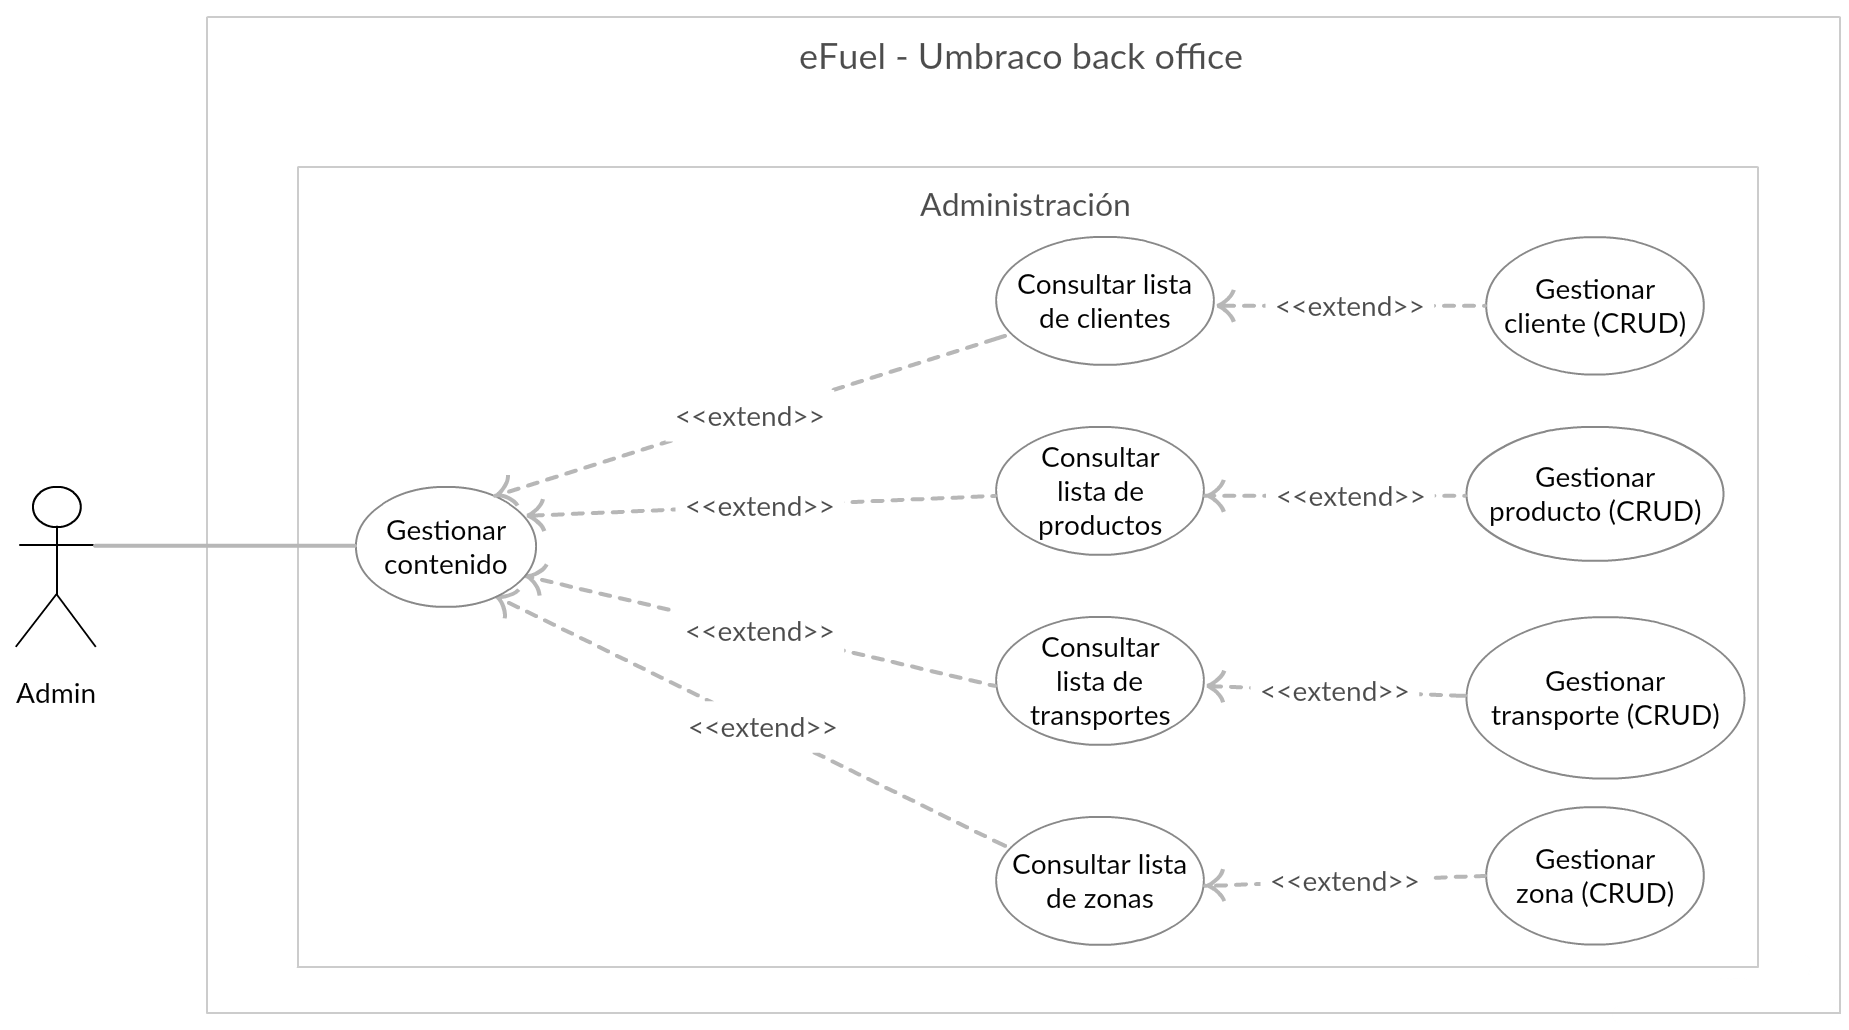
\includegraphics[width=\textwidth]{cu_admin_administracion.png}
    \caption{Casos de Uso Back office - Módulo Administración}
    \label{fig:cu_admin_administracion}
\end{figure}

\newpage
La Figura \ref{fig:cu_admin_pedidos_pagos} muestra los casos de uso del actor \textit{Admin} de los Módulos de Pedidos y Pagos.
\begin{figure}[H]
    \centering
    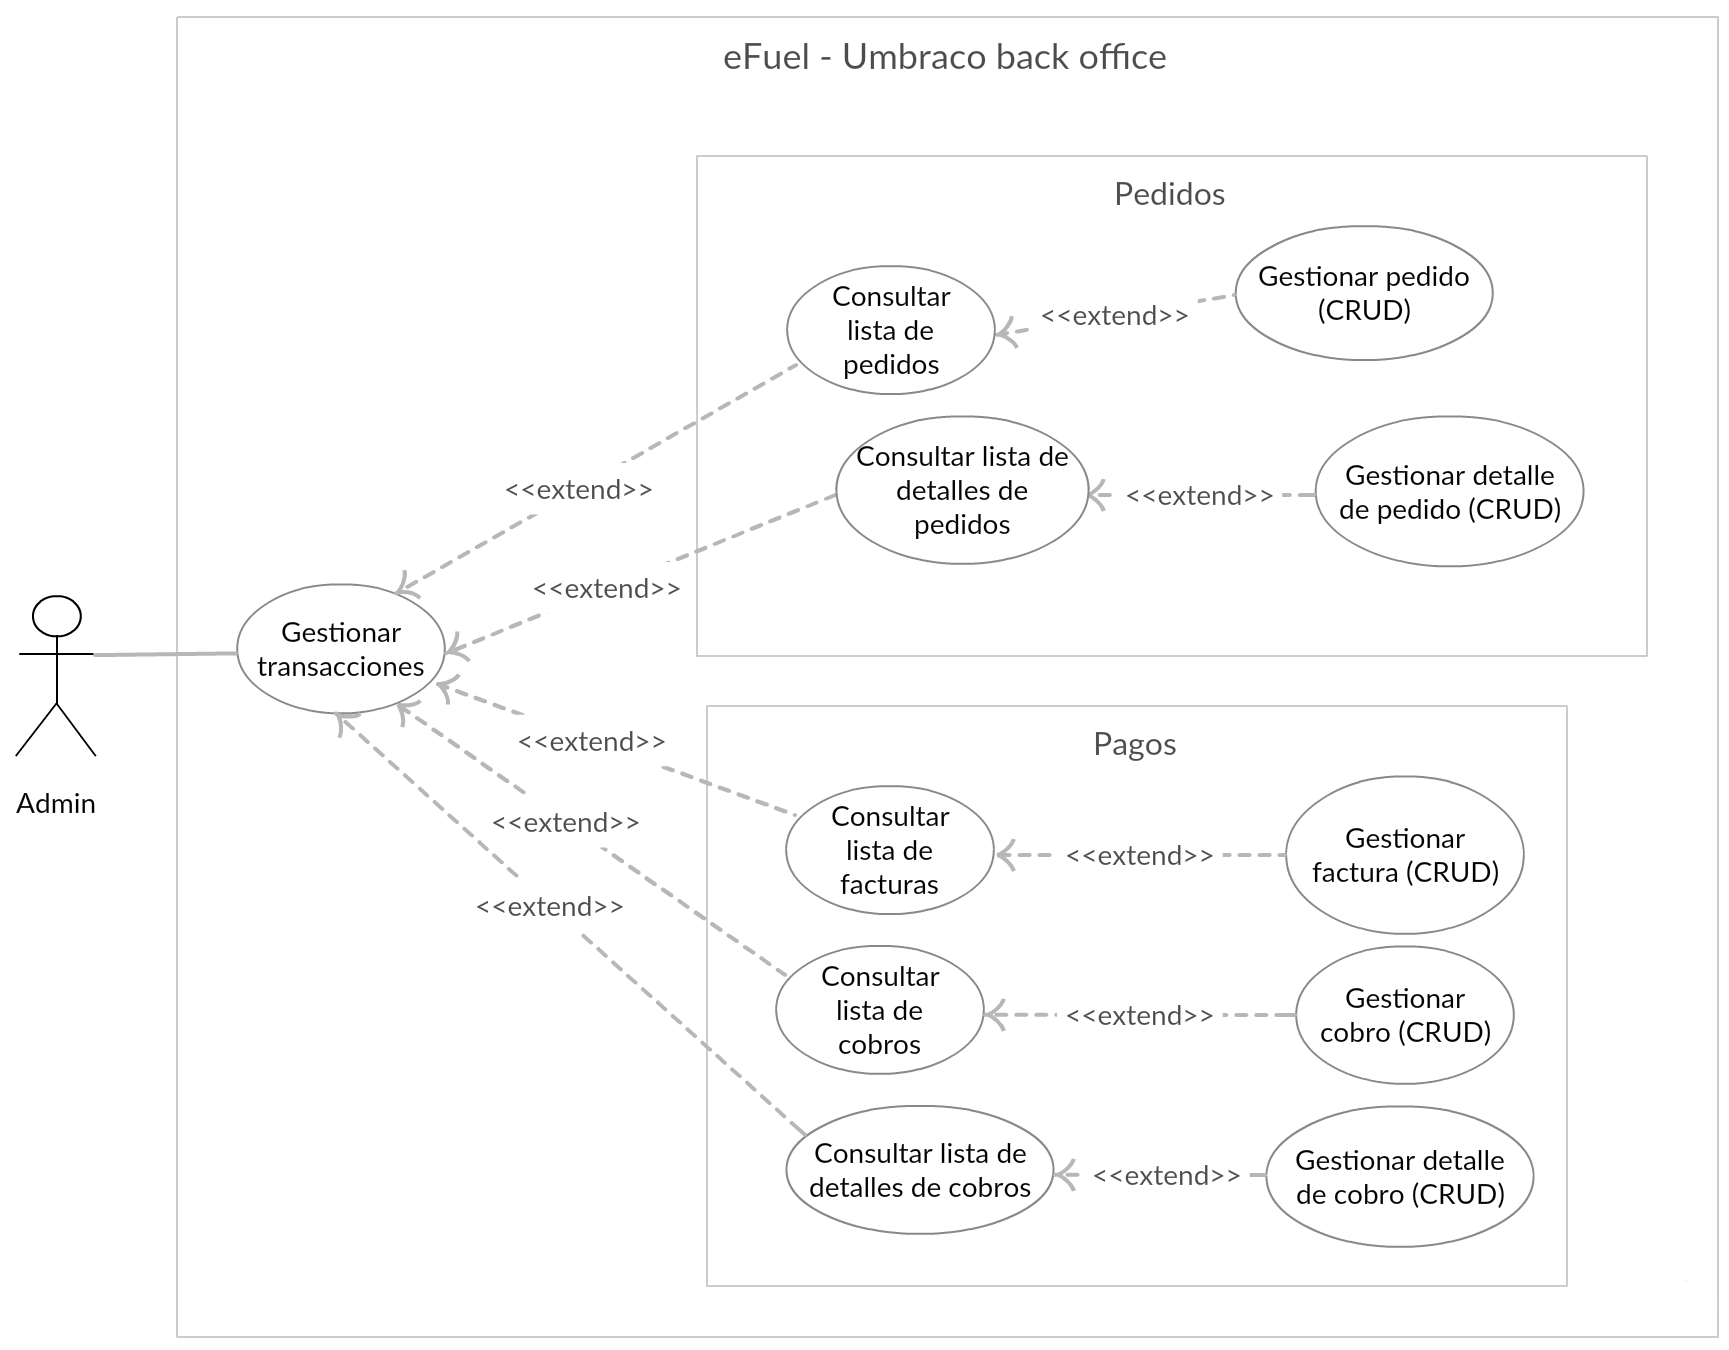
\includegraphics[width=0.9\textwidth]{cu_admin_pedidos_pagos.png}
    \caption{Casos de Uso Back office - Módulos Pedidos y Pagos}
    \label{fig:cu_admin_pedidos_pagos}
\end{figure}

\newpage
La Figura \ref{fig:cu_admin_seguridad} muestra los casos de uso del actor \textit{Admin} del Módulo de Seguridad.
\begin{figure}[H]
    \centering
    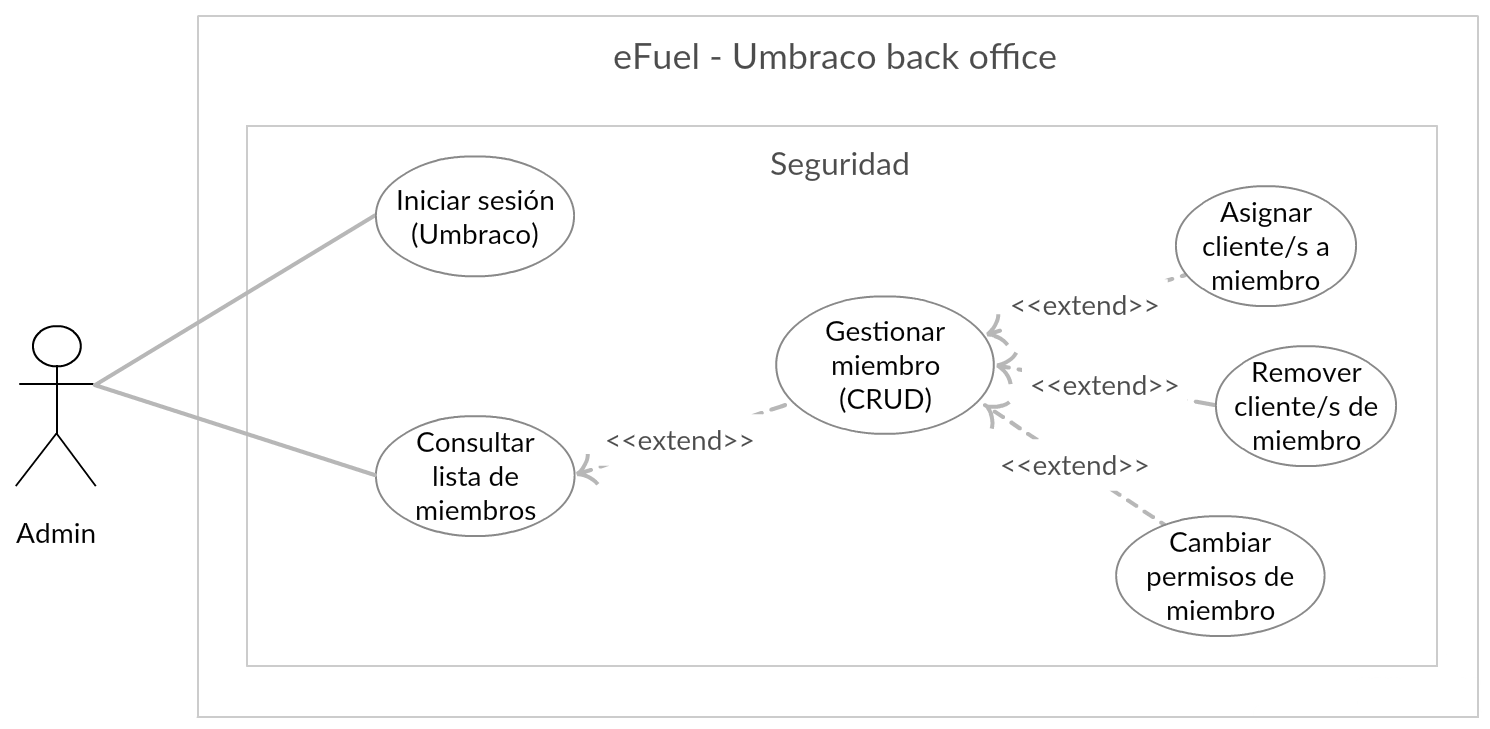
\includegraphics[width=0.9\textwidth]{cu_admin_seguridad.png}
    \caption{Casos de Uso Back office - Módulo Seguridad}
    \label{fig:cu_admin_seguridad}
\end{figure}
\vspace*{\fill}

\newpage
La Figura \ref{fig:cu_customer_staff_pedidos} muestra los casos de uso de los actores \textit{Staff} y \textit{Customer} de los Módulos de Pedidos y Seguridad.
\begin{figure}[H]
    \centering
    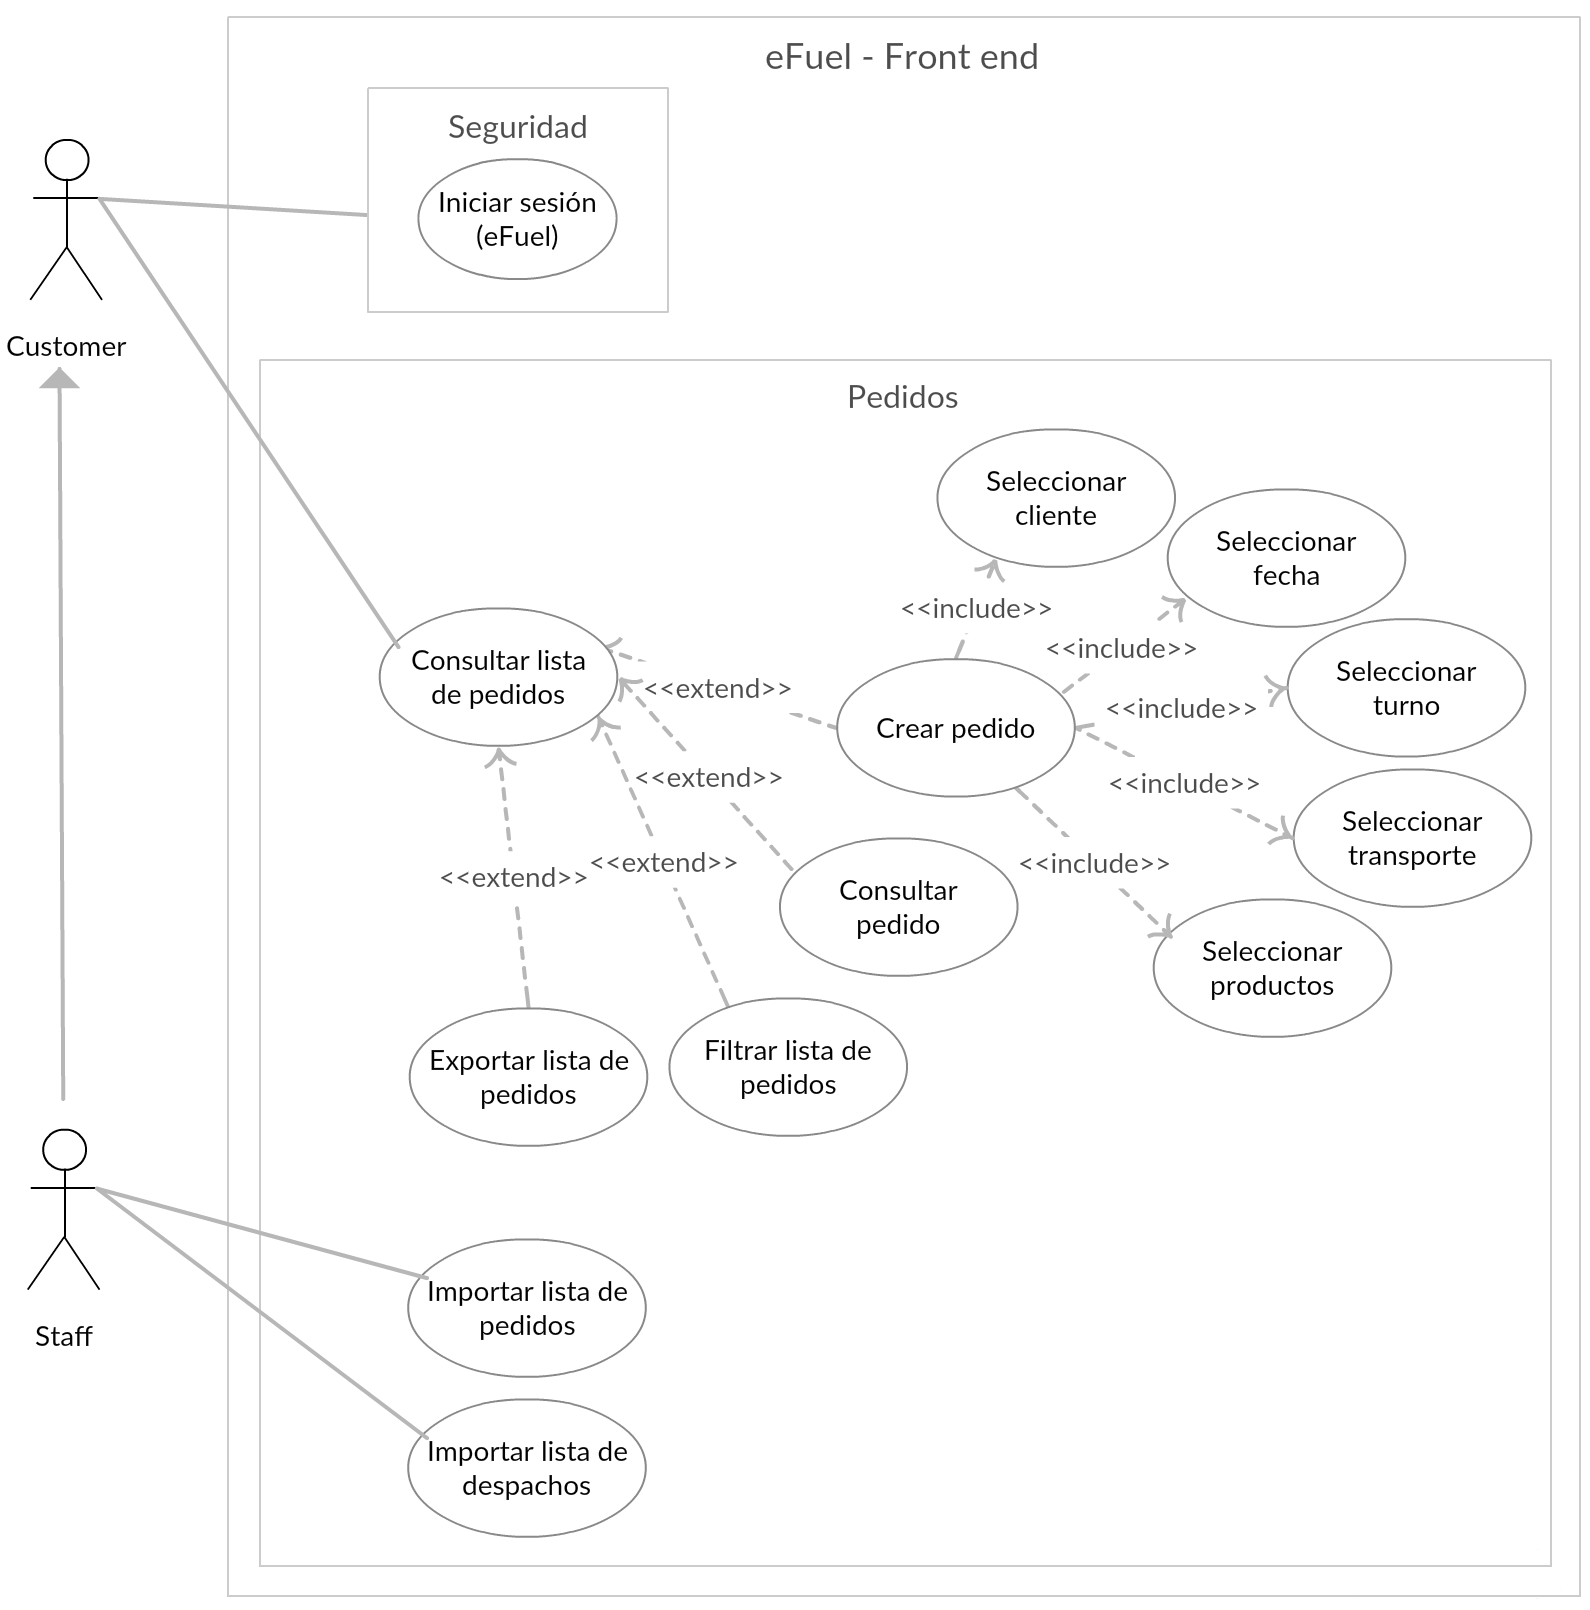
\includegraphics[width=\textwidth]{cu_customer_staff_pedidos_seguridad.png}
    \caption{Casos de Uso Front end - Módulos Pedidos y Seguridad}
    \label{fig:cu_customer_staff_pedidos}
\end{figure}
\vspace*{\fill}

\newpage
La Figura \ref{fig:cu_customer_staff_pagos} muestra los casos de uso de los actores \textit{Staff} y \textit{Customer} del Módulo de Pagos.
\begin{figure}[H]
    \centering
    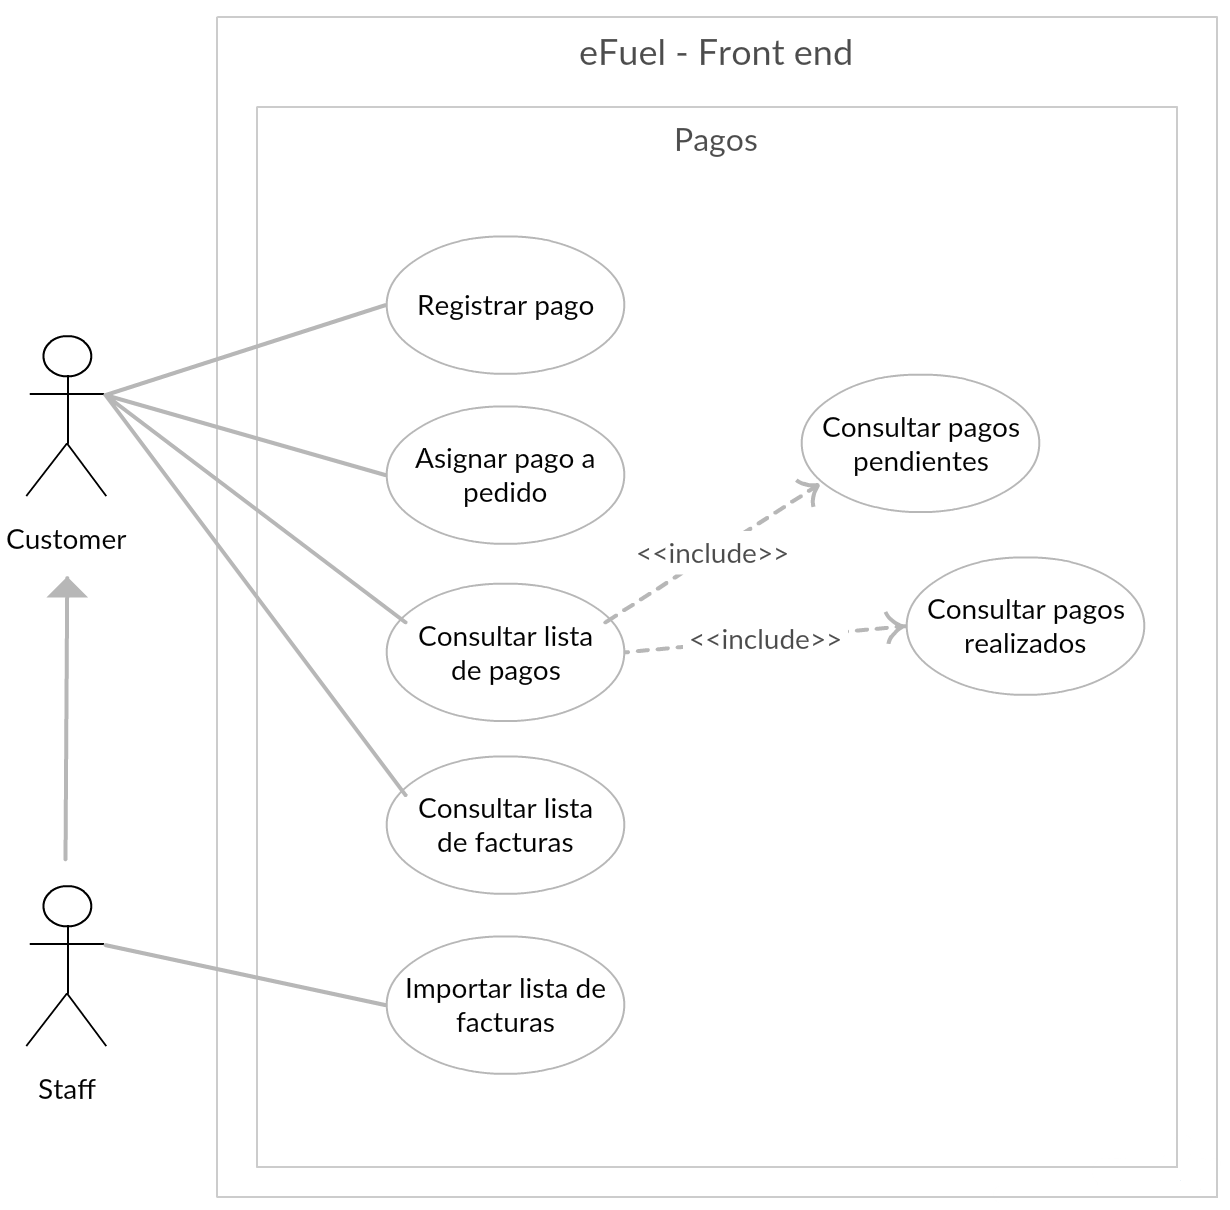
\includegraphics[width=\textwidth]{cu_customer_staff_pagos.png}
    \caption{Casos de Uso Front end - Módulo Pagos}
    \label{fig:cu_customer_staff_pagos}
\end{figure}
\vspace*{\fill}

\newpage
La Figura \ref{fig:cu_customer_staff_administracion} muestra los casos de uso de los actores \textit{Staff} y \textit{Customer} del Módulo de Administración.
\begin{figure}[H]
    \centering
    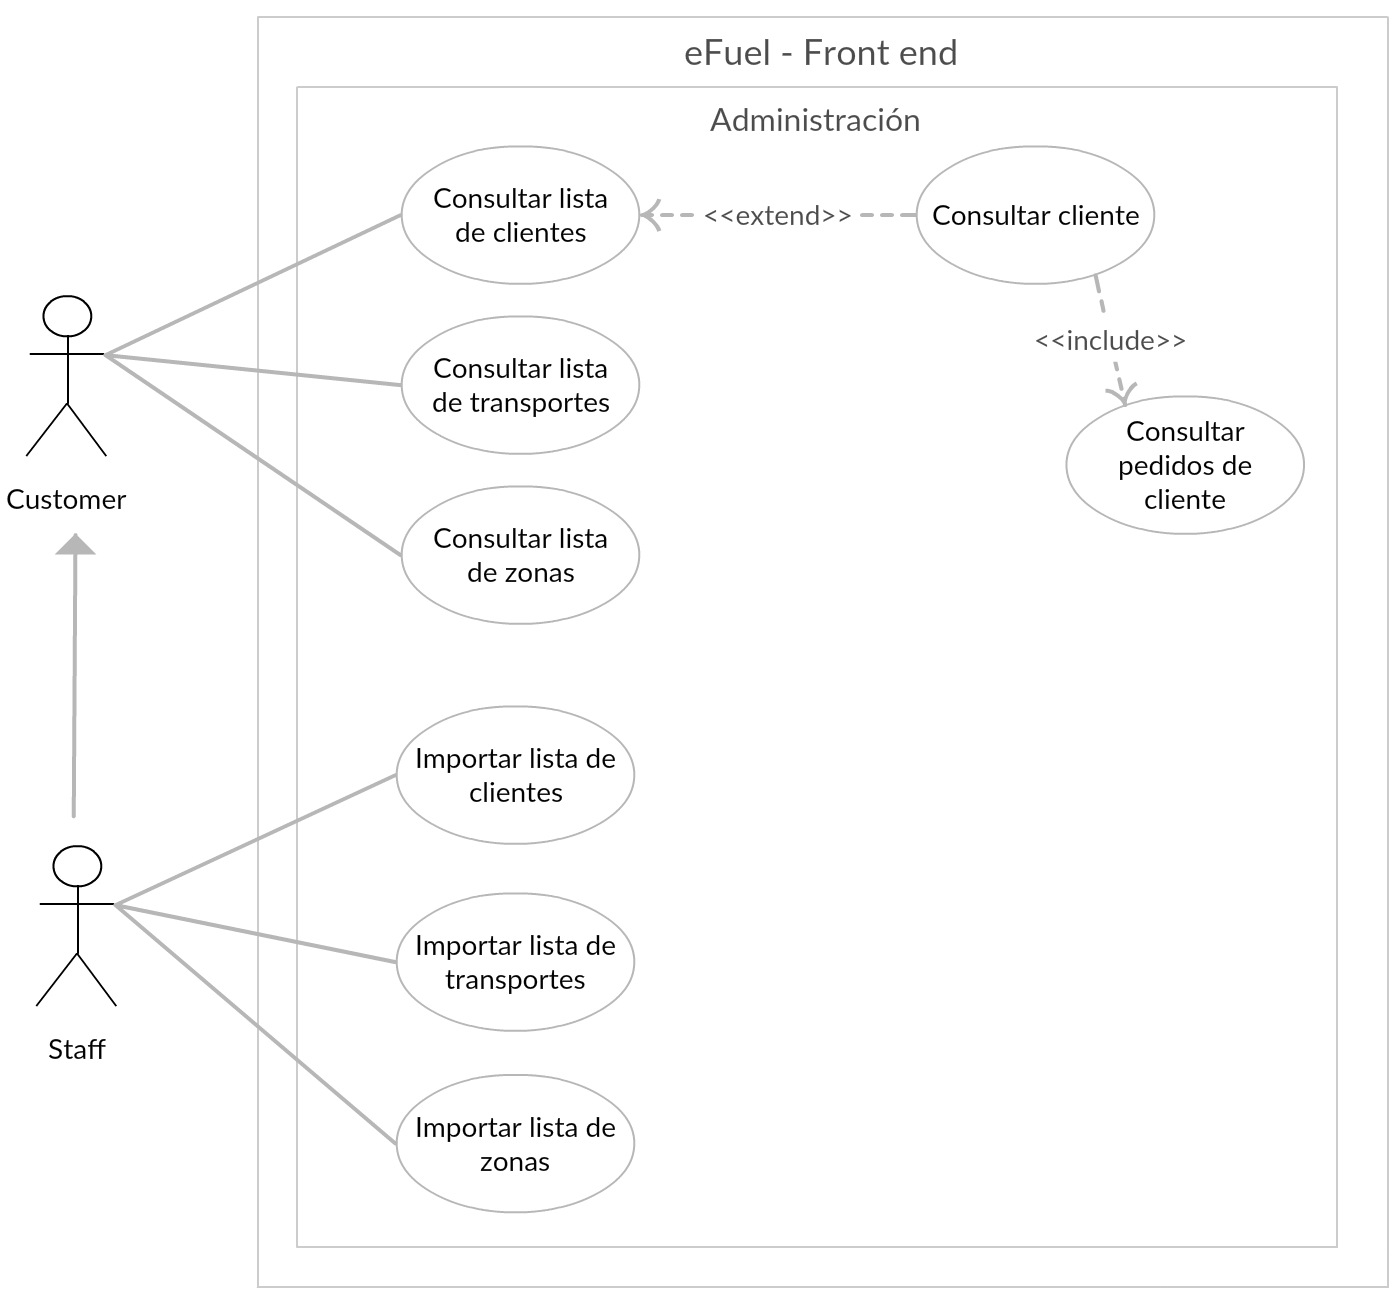
\includegraphics[width=\textwidth]{cu_customer_staff_administracion.png}
    \caption{Casos de Uso Front end - Módulo Administración}
    \label{fig:cu_customer_staff_administracion}
\end{figure}

\newpage
\paragraph{Vista Lógica} se muestran 2 diagramas que describen, de manera estática, la estructura del sistema y su interacción con entidades externas.

\subparagraph*{Diagrama Conceptual (Modelo de Dominio)} este diagrama muestra la interacción de eFuel con sistemas y agentes externos.
\begin{figure}[H]
    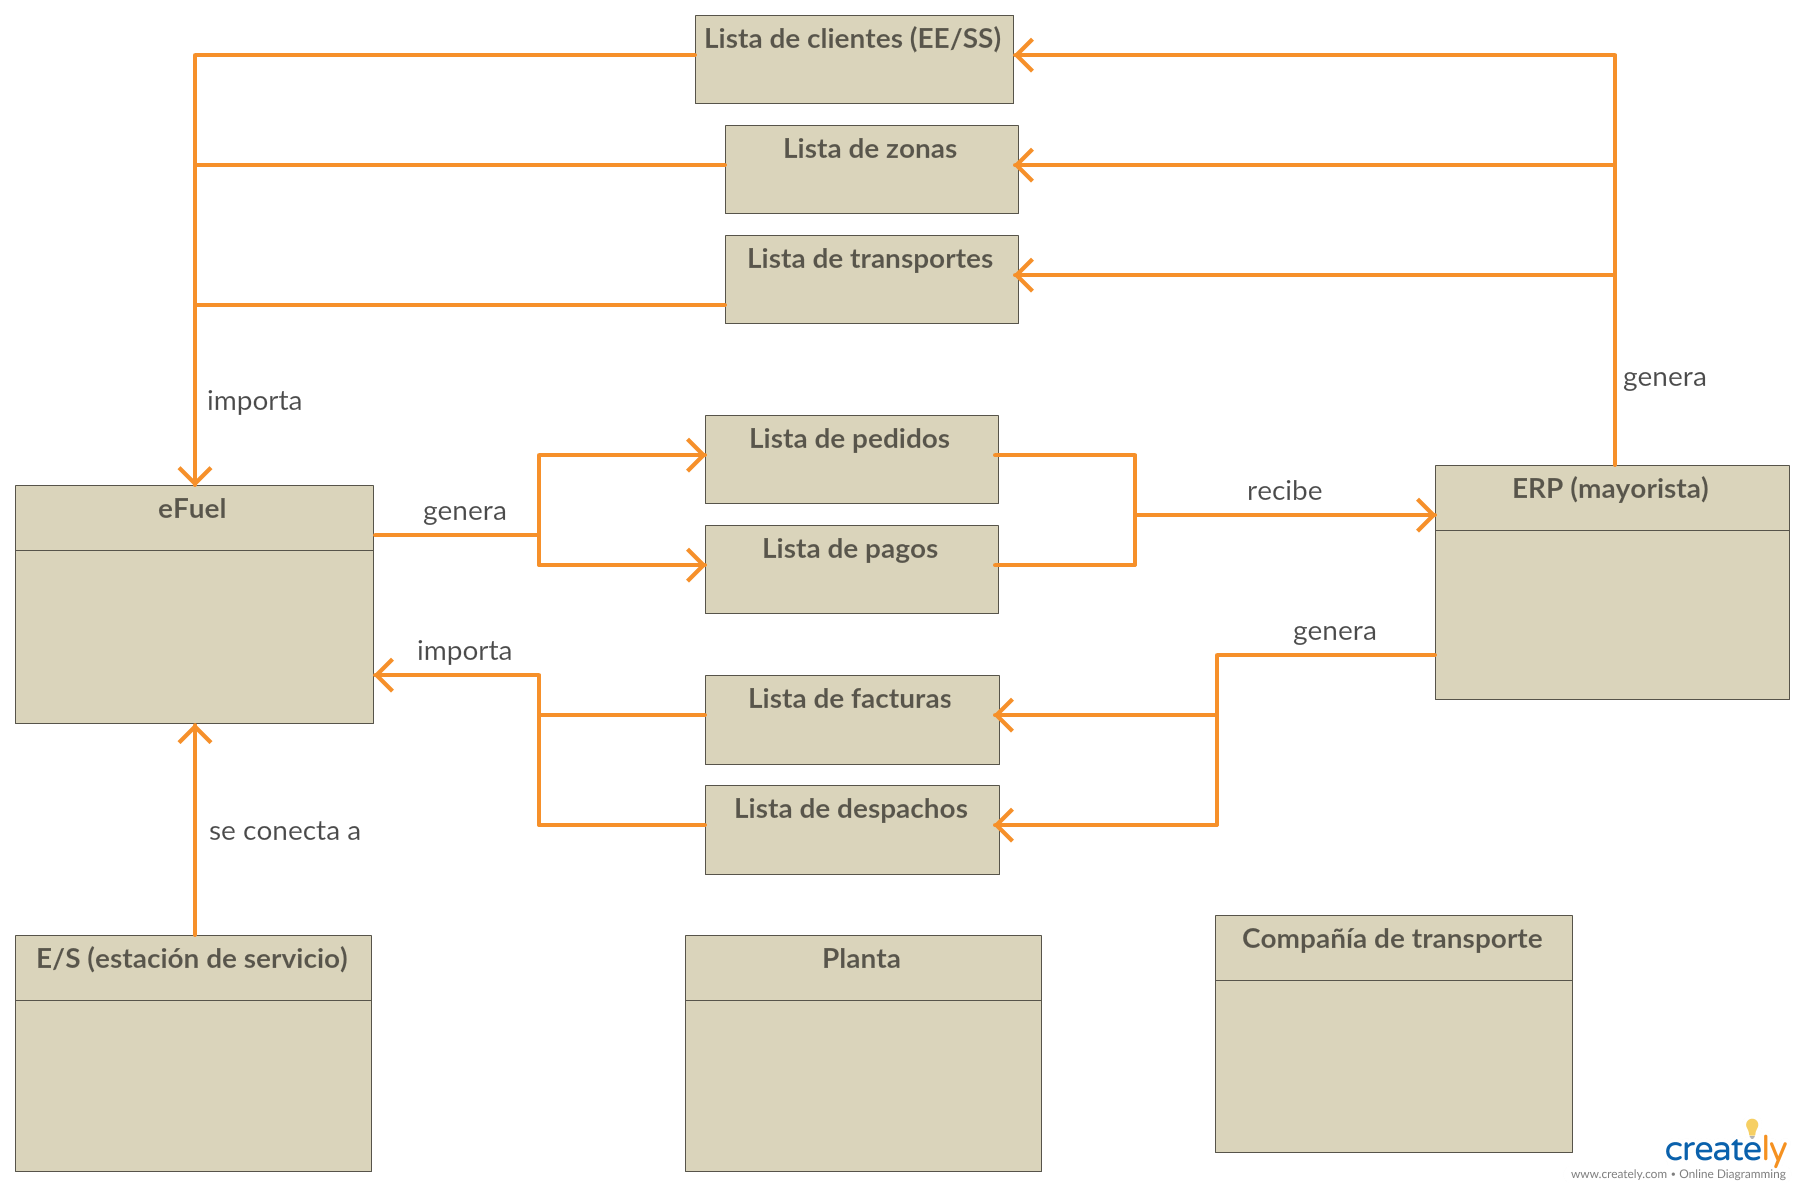
\includegraphics[width=\textwidth]{domain_model.png}
    \caption{Modelo de Dominio}
    \label{fig:domain_model}
    \centering
\end{figure}

\subparagraph*{Diagrama de Clases} a continuación se muestra un diagrama donde están representadas las principales entidades del sistema y las relaciones entre ellas. Las tablas con los bordes punteados son Doctypes de Umbraco representados como clases y los de línea continua son las clases principales del sistema (no son Doctypes de Umbraco).

\begin{figure}[H]
    \centering
    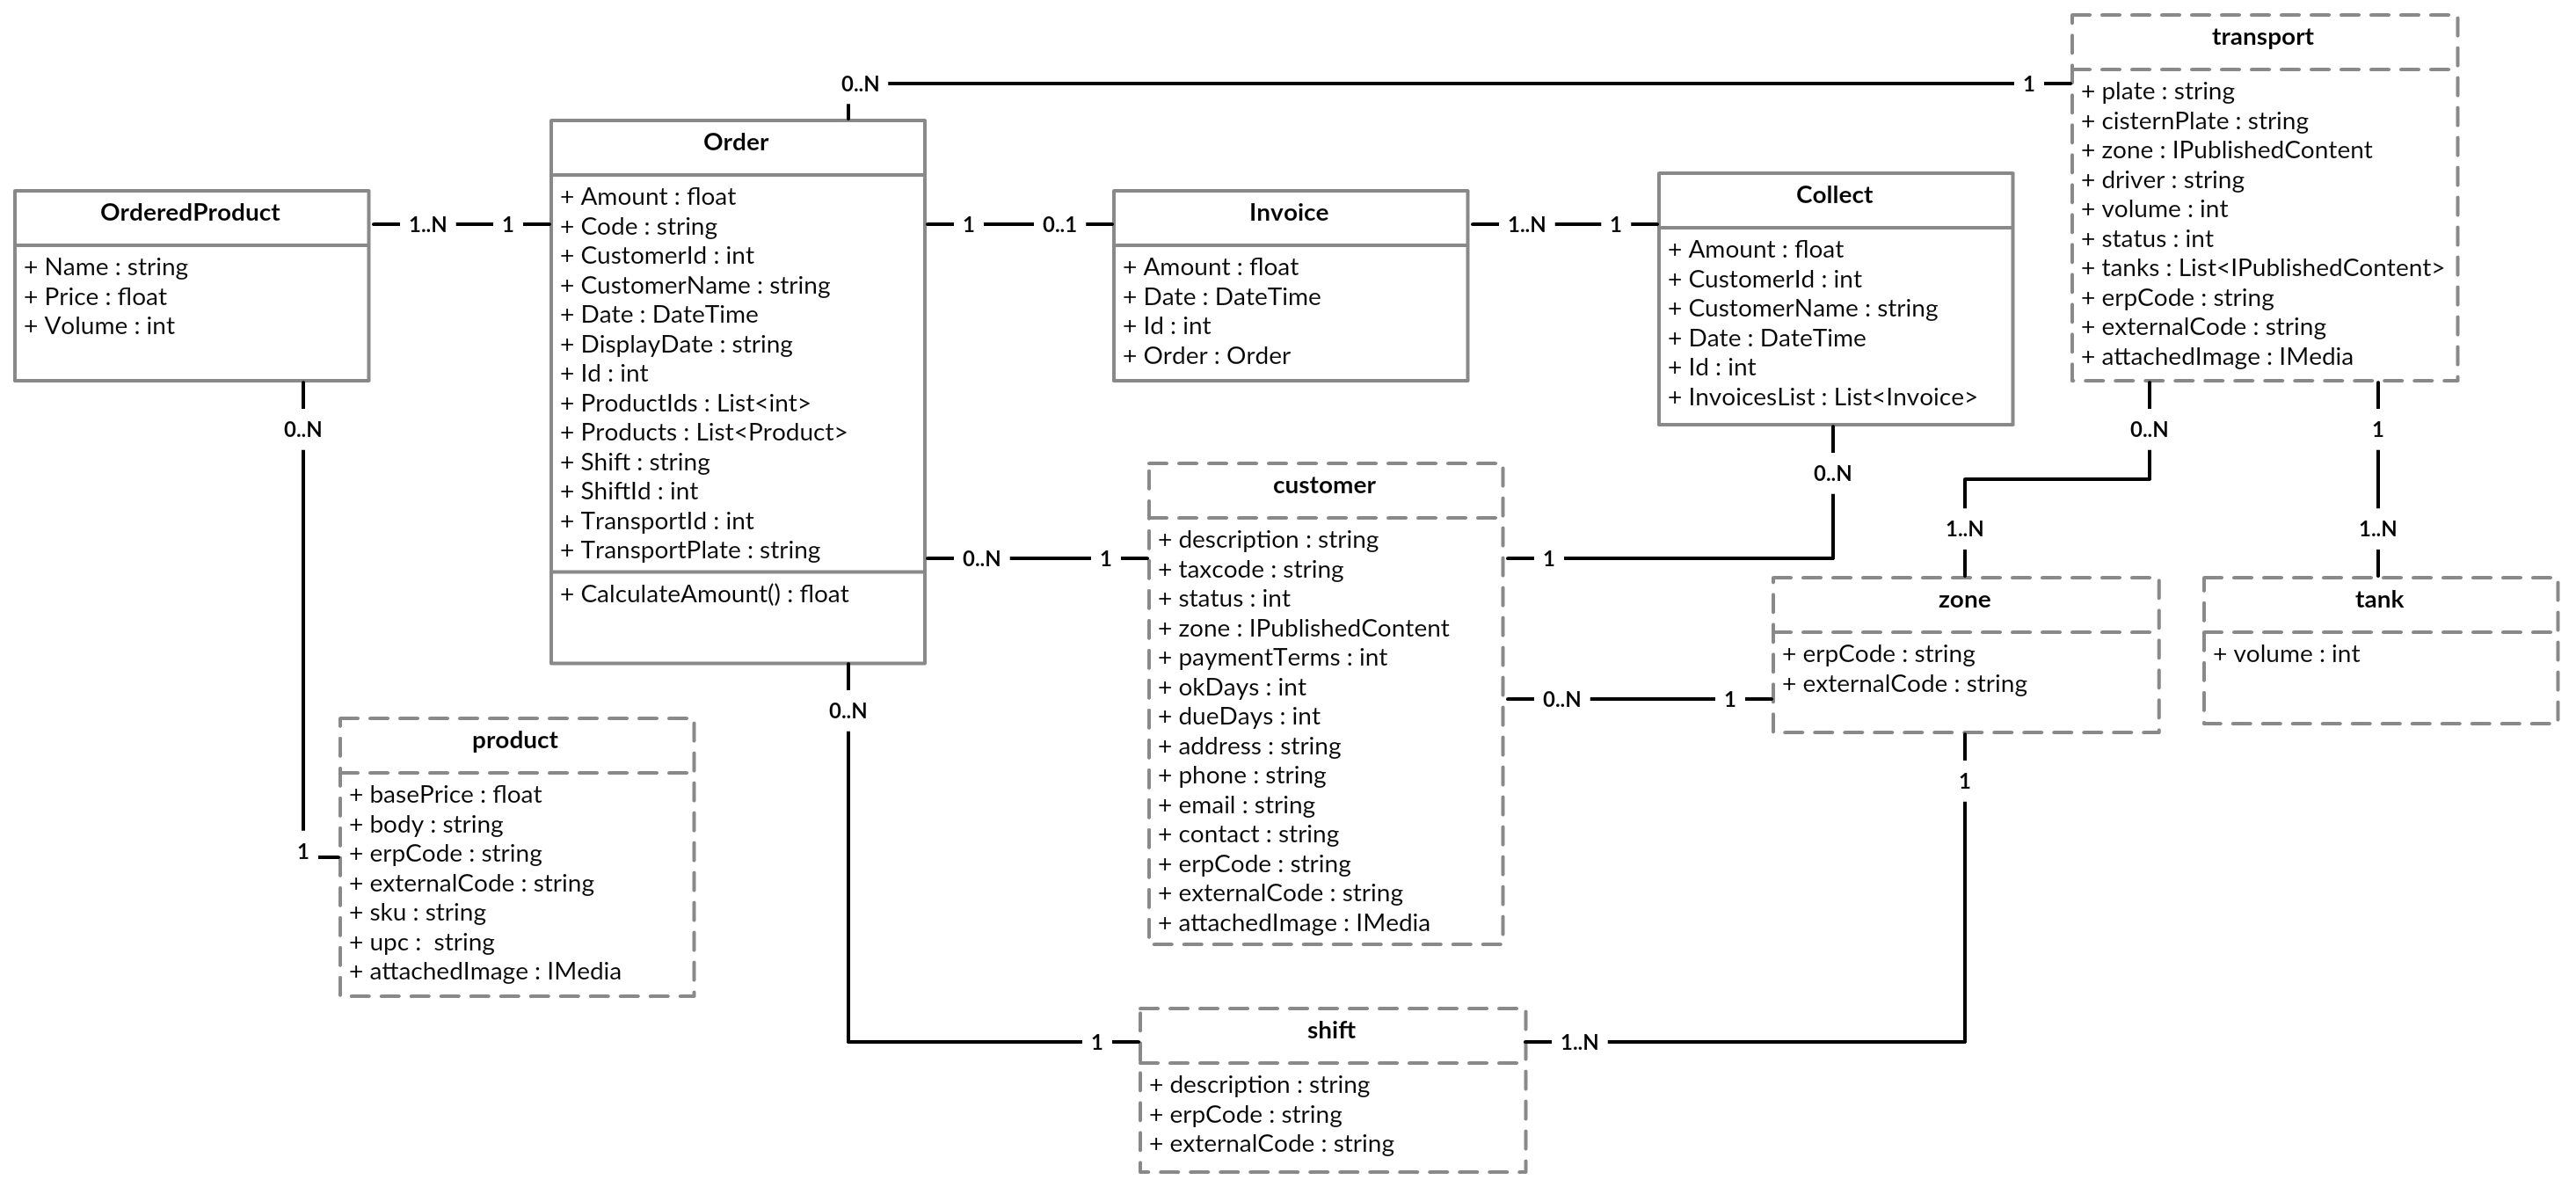
\includegraphics[width=0.7\textwidth]{class_diagram.png}
    \caption{Diagrama de Clases de las entidades principales}
    \label{fig:class_diagram_main}
\end{figure}

\paragraph{Vista de Implantación} esta vista muestra los dispositivos y artefactos necesarios para la implantación del sistema.

\begin{figure}[H]
    \centering
    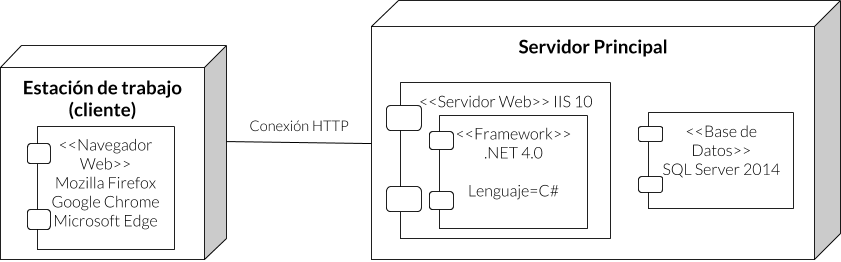
\includegraphics[width=\textwidth]{diagrama_implantacion.png}
    \caption{Diagrama de Despliegue}
    \label{fig:diagrama_implantacion}
\end{figure}

\paragraph{Vista de Implementación} esta vista hace énfasis sobre la organización de los módulos de software en el ambiente de desarrollo, en la terminología de Visual Studio (introducida en el Marco Tecnológico) estos módulos se conocen como "proyectos". La arquitectura de software desarrollada para esta vista se diseñó basándose en la arquitectura MVC. A continuación se muestra una descripción de los proyectos de la solución de Visual Studio, seguido por el Diagrama de Componentes del sistema.

\subparagraph*{Módulos de eFuel} El proyecto está compuesto por 3 módulos:
\begin{itemize}
    \item \texttt{EF\_API}: contiene los controladores usados para implementar los servicios web. Estos controladores heredan de la clase \texttt{UmbracoApiController} y su función es buscar datos (normalmente listas) y devolverlos en formato JSON al cliente. Se creó un controlador por cada entidad principal del sistema (clientes, transportes, órdenes, etc).
    \item \texttt{EF\_Core}: contiene los controladores del patrón MVC, los manejadores de rutas (Route Handlers) para éstos y los modelos que sirven para interactuar con la base de datos. Los controladores de este módulo heredan de la clase \texttt{SurfaceController} y su función es, básicamente, buscar datos y devolver vistas. Hay un controlador por cada tipo de entidad principal del sistema (clientes, transportes, órdenes, etc).
    \item \texttt{EF\_Miscelaneous}: contiene todos los archivos de la Vista del patrón MVC, esto es, las vistas (HTML), los archivos de estilo (CSS) y los scripts del front end (JavaScript). Además contiene los archivos de configuración de Fluidity.
\end{itemize}

\subparagraph*{Diagrama de Componentes} el usuario introduce un URL, el componente \texttt{eFuel\-RouteHandler} se encarga de asociar un URL con un controlador para llamarlo, el controlador realiza sus tareas y devuelve una vista (en el caso de los \texttt{SurfaceController}) o datos (en el caso de los \texttt{UmbracoApiController}).

\begin{figure}[H]
    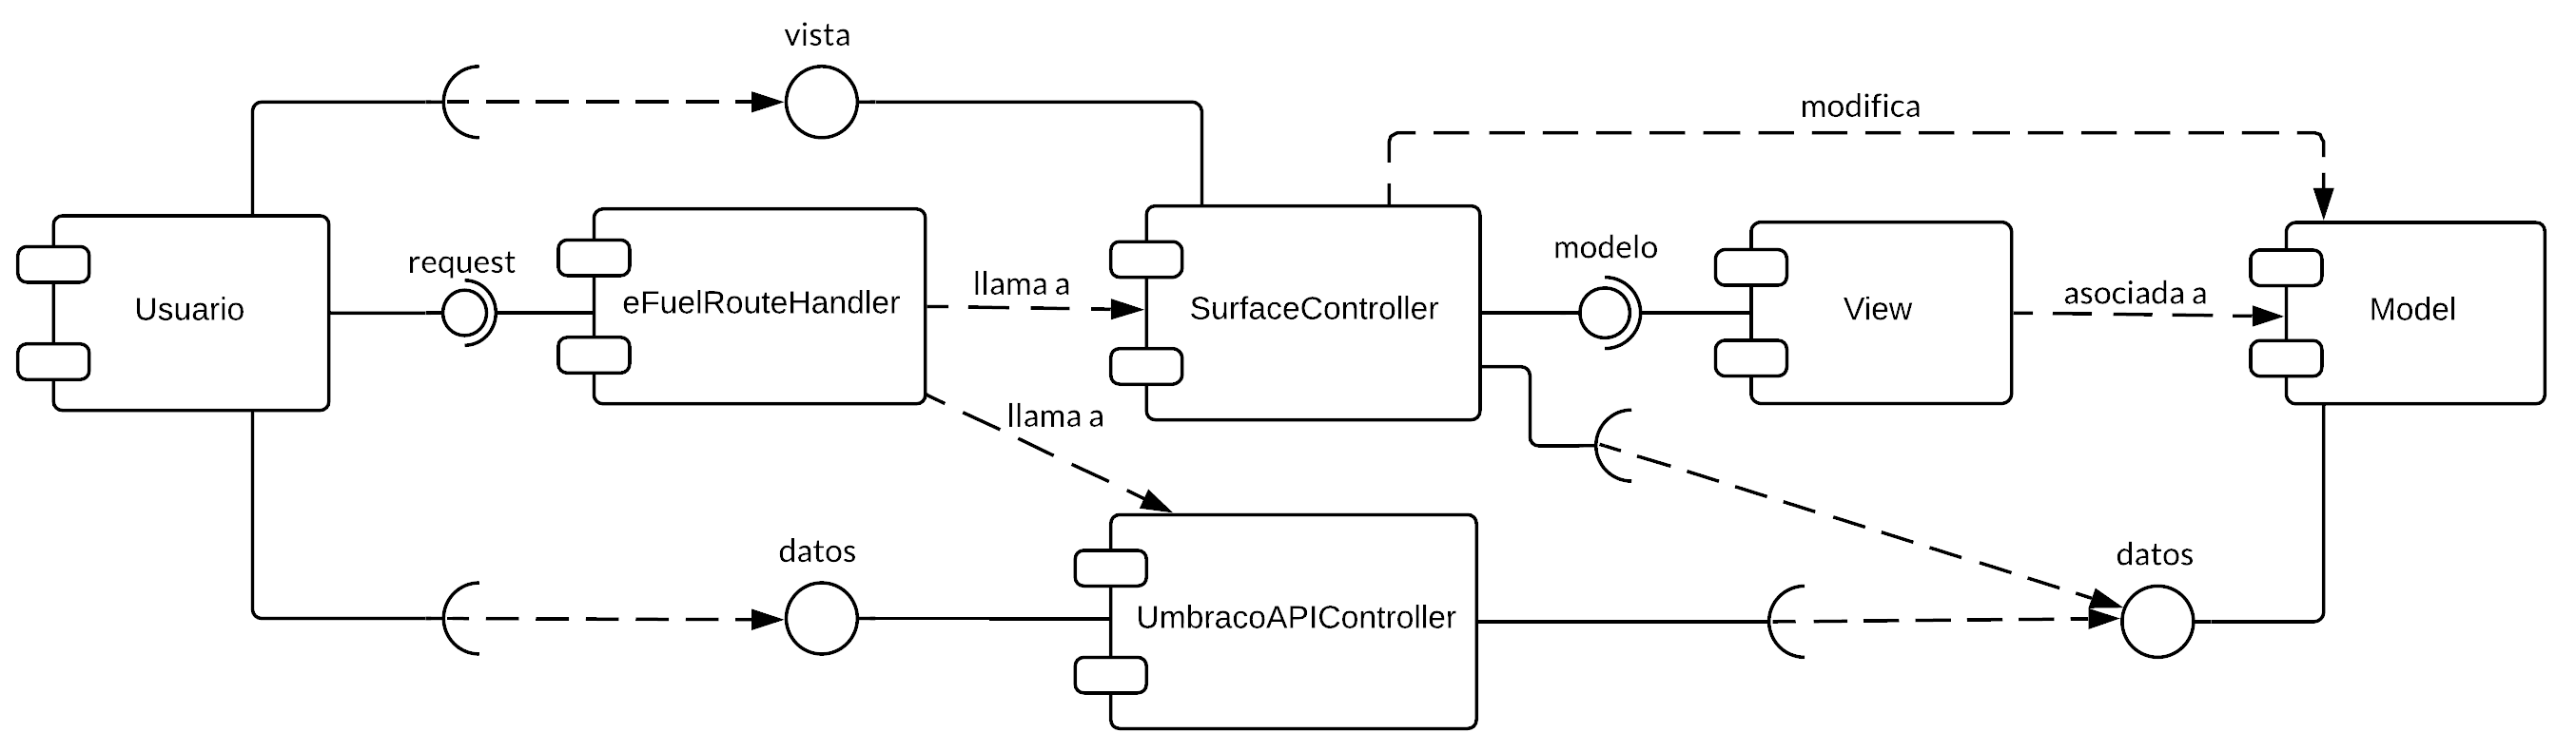
\includegraphics[width=\textwidth]{component_diagram.png}
    \caption{Diagrama de Componentes}
    \label{fig:component_diagram}
    \centering
\end{figure}

\paragraph{Componentes de Umbraco} se documenta la estructura de los componentes desarrollados en el back office de Umbraco. Primero se muestra una tabla con la lista de todas las vistas desarrolladas para el sistema, luego una tabla con los Doctypes y finalmente una tabla con los Data Types diseñados para eFuel.

\begin{longtable}{ | p{5.5em} | p{7em} | p{15em} | c | }
    \hline
    \rowcolor{gray!30}
    \multicolumn{1}{|c|}{Modelo} &
    \multicolumn{1}{|c|}{Nombre} &
    \multicolumn{1}{|c|}{Descripción} &
    \multicolumn{1}{|c|}{Partial View} \\
    \hhline{====}
    \endhead

    \hline
    \endfoot

    \endlastfoot

    Customer
        & Dashboard & Panel con las acciones principales que se pueden realizar sobre los clientes & - \\
    \cline{2-4}
        & Details & Información detallada de un cliente & - \\
    \cline{2-4}
        & Edit & Formulario para editar la información de un cliente & \checkmark \\
    \cline{2-4}
        & List & Tabla con todos los clientes que puede ver el usuario & \checkmark \\
    \hline

    Home
        & Dashboard & Mensaje de bienvenida (eventualmente debe mostrar las opciones más importantes del sistema) & - \\
    \hline

    Invoice
        & Dashboard & Panel con las acciones principales que se pueden realizar sobre las facturas & - \\
    \cline{2-4}
        & List & Tabla con las facturas & \checkmark \\
    \hline

    Membership
        & Index & Página de inicio de sesión & - \\
    \hline

    Order
        & Create & Formulario para crear un nuevo pedido & \checkmark \\
    \cline{2-4}
        & Dashboard & Panel con las acciones principales que se pueden realizar sobre los pedidos & - \\
    \cline{2-4}
        & Details & Información detallada de un pedido & - \\
    \cline{2-4}
        & List & Tabla con todos los pedidos que puede ver el usuario junto con los filtros y opciones de exportar la lista, crear un nuevo pedido y filtrar la lista de pedidos & \checkmark \\
    \hline

    Shared
        & AppTitle & Título de la página actual & \checkmark \\
    \cline{2-4}
        & Breadcrumbs & Cadena de enlaces a las páginas superiores a la página actual & \checkmark \\
    \cline{2-4}
        & LoginForm & Formulario de inicio de sesión & \checkmark \\
    \cline{2-4}
        & LogoutButton & Botón de cerrar sesión & \checkmark \\
    \cline{2-4}
        & Master & Estructura del sitio que es común a todas las páginas del sitio (excepto la página de inicio de sesión). Barra de navegación, barra lateral, título, etc. & - \\
    \cline{2-4}
        & Navbar & Barra de navegación superior & \checkmark \\
    \cline{2-4}
        & Sidebar & Barra de navegación lateral, contiene las secciones del sitio & \checkmark \\
    \hline

    Transport
        & Dashboard & Panel con las acciones principales que se pueden realizar sobre los transportes & - \\
    \cline{2-4}
        & Details & Información detallada de un transporte & - \\
    \cline{2-4}
        & Import & Formulario para importar una lista transportes & \checkmark \\
    \cline{2-4}
        & List & Tabla con los transportes que puede ver el usuario & \checkmark \\
    \hline

    Zone
        & Dashboard & Panel con las acciones principales que se pueden realizar sobre las zonas & - \\
    \cline{2-4}
        & Import & Formulario para importar una lista zonas & \checkmark \\
    \cline{2-4}
        & List & Tabla con las zonas que puede ver el usuario & \checkmark \\
    \hline

    \caption{Vistas del front end}
    \label{table:vistas}
\end{longtable}

\begin{longtable}{ | p{5em} | l | l | }
    \hline
    \rowcolor{gray!30}
    \multicolumn{1}{|c|}{Doctype} &
    \multicolumn{1}{|c|}{Propiedades} &
    \multicolumn{1}{|c|}{Datatype} \\
    \hline
    \endhead

    \hline
    \endfoot

    \endlastfoot

    Cliente
        & Descripción & Textarea \\
        \cline{2-3}
        & Código de impuestos & Textstring \\
        \cline{2-3}
        & Estado & Customer status \\
        \cline{2-3}
        & Zona & Zone node picker \\
        \cline{2-3}
        & Forma de pago & Payment terms \\
        \cline{2-3}
        & Ok days & Numeric \\
        \cline{2-3}
        & Due days & Numeric \\
        \cline{2-3}
        & Dirección & Textstring \\
        \cline{2-3}
        & Teléfono & Textstring \\
        \cline{2-3}
        & Correo & Email address \\
        \cline{2-3}
        & Contacto & Textstring \\
        \cline{2-3}
        & Código ERP & Textstring \\
        \cline{2-3}
        & Código externo & Textstring \\
        \cline{2-3}
        & Imagen & Attached images \\
    \hline

    Producto
        & Precio base & Decimal \\
        \cline{2-3}
        & Descripción & Textarea \\
        \cline{2-3}
        & Código ERP & Textstring \\
        \cline{2-3}
        & Código externo & Textstring \\
        \cline{2-3}
        & SKU & Textstring \\
        \cline{2-3}
        & EAN/UPC & EAN-UPC \\
        \cline{2-3}
        & Imagen & Attached images \\
    \hline

    Tanque
        & Volumen & Numeric \\
    \hline

    Transporte
        & Placa chuto & Textstring \\
        \cline{2-3}
        & Placa cisterna & Textstring \\
        \cline{2-3}
        & Zona & Zone node picker \\
        \cline{2-3}
        & Nombre del conductor & Textstring \\
        \cline{2-3}
        & Volumen total & Numeric \\
        \cline{2-3}
        & Estado & Transport status \\
        \cline{2-3}
        & Tanques & Tank list \\
        \cline{2-3}
        & Código ERP & Textstring \\
        \cline{2-3}
        & Código externo & Textstring \\
        \cline{2-3}
        & Imagen & Attached images \\
    \hline

    Turno
        & Descripción & Textstring \\
        \cline{2-3}
        & Código ERP & Textstring \\
        \cline{2-3}
        & Código externo & Textstring \\
    \hline

    Zona
        & Código ERP & Textstring \\
        \cline{2-3}
        & Código externo & Textstring \\
    \hline

    \caption{Doctypes}
    \label{table:doctypes}
\end{longtable}

\begin{longtable}{  l | l  }
    \hline\hline
    \rowcolor{gray!30}
    \textbf{Datatype} & \textbf{Uso} \\
    \hline\hline
    \endhead

    \hline
    \endfoot

    \endlastfoot

    Collect picker & Seleccionar un cobro \\
    Customer picker & Seleccionar un cliente \\
    Invoice picker & Seleccionar una factura \\
    Order picker & Seleccionar un pedido \\
    Product picker & Seleccionar un producto \\
    Shift picker & Seleccionar un turno \\
    Tank picker & Seleccionar un tanque \\
    Transport picker & Seleccionar un transporte del árbol de contenido \\
    Customer node picker & Seleccionar el nodo de un cliente del árbol de contenido \\
    Zone node picker & Seleccionar el nodo de una zona del árbol de contenido \\
    Attached images & Seleccionar una imagen \\
    Customer status & Elegir uno de los estados del cliente \\
    EAN-UPC & Introducir el código EAN o UPC de un producto \\
    Email address & Introducir un correo electrónico \\
    On Off & Elegir uno de 2 estados: on u off \\
    Payment terms & ELegir una forma de pago \\
    Tank list & Agregar o eliminar tanques a un transporte \\
    Textstring max65 & Introducir texto de máximo 65 caracteres \\
    Transport status & Seleccionar el estado de un transporte \\

    \hline

    \caption{Datatypes}
    \label{table:datatypes}
\end{longtable}

\paragraph{Vista de Datos} se documenta la estructura de las entidades creadas fuera de Umbraco para la base de datos.
\begin{figure}[H]
    \centering
    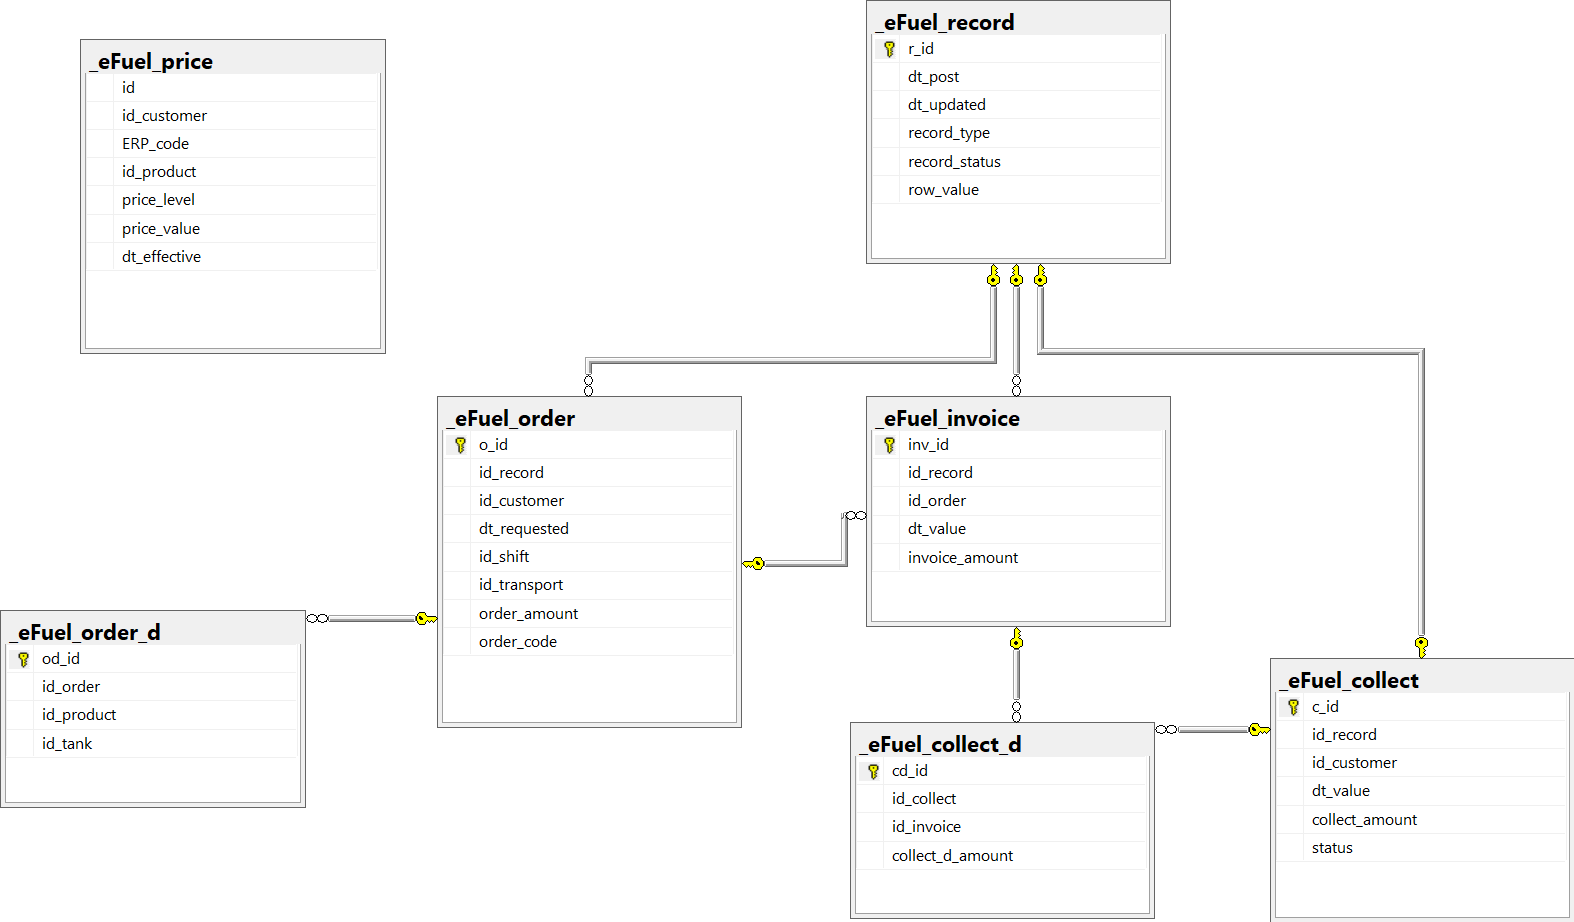
\includegraphics[width=\textwidth]{er_diagram.png}
    \caption{Diagrama ER}
    \label{fig:er_diagram}
\end{figure}